% Slides of the tables and figures of ../latency_memory_loss_moo/main.tex and the tables of
% ../compression/benchmarks/report.tex, one per slide. Generated by make_slides.py; build from this folder:
% latexmk -pdf slides.tex
\documentclass[aspectratio=169,10pt]{beamer}
\usetheme{default}
\setbeamertemplate{navigation symbols}{}
\setbeamertemplate{footline}[frame number]
\setbeamerfont{frametitle}{size=\large}
\setbeamertemplate{caption}[numbered]
\setbeamerfont{caption}{size=\scriptsize}
\setbeamercolor{caption}{fg=black!70}
\setbeamercolor{caption name}{fg=black}
\usepackage[T1]{fontenc}
\usepackage{lmodern}
\usepackage{amsmath,amssymb}
\usepackage{booktabs}
\usepackage{array}
\usepackage{graphicx}
\usepackage{adjustbox}
\usepackage{subcaption}
\usepackage{tikz}
\usetikzlibrary{arrows.meta,positioning}
\usepackage{xr}
\externaldocument[R-]{../latency_memory_loss_moo/main}  % R-sec:..., R-eq:...: the report's numbers
\externaldocument[B-]{../compression/benchmarks/report}  % B-sec:...: the benchmark report's
\renewcommand{\cite}[1]{}
\captionsetup[subfigure]{font=scriptsize}

\newcommand{\dloss}{\Delta\mathcal{L}}
\newcolumntype{P}[1]{>{\raggedright\arraybackslash}p{#1}}
\definecolor{cprep}{HTML}{7A8699}
\definecolor{csearch}{HTML}{2A78D6}
\definecolor{ceval}{HTML}{1BAF7A}
\definecolor{cfinal}{HTML}{EB6834}
\newcommand{\us}{\,$\mu$s}

\title{Hardware-Aware Multi-Objective Compression of Language Models}
\subtitle{Tables and figures}
\author{Rasa Khosrowshahli}
\date{November 2026}

\begin{document}
\begin{frame}
\titlepage
\end{frame}

\begin{frame}{Motivation}{}
\begin{table}
\centering
\begin{adjustbox}{width=\linewidth, totalheight=0.64\textheight, keepaspectratio, center}
\centering
\small
\begin{tabular}{lccc}
\toprule
Weights of an $8704\times2176$ matrix (d34 MLP) & Zeros & Batch 1 (\us) & Batch 2048 (\us) \\
\midrule
Original bf16                              & 0\%  & 175.6   & 3092 \\
UBQ, $k=256$                               & 1\%  & 171.3   & 3053 \\
UBQ, $k=16$                                & 21\% & 175.9   & 3055 \\
UBQ, $k=3$ with interval pruning           & 93\% & 176--181 & 3059--3140 \\
\bottomrule
\end{tabular}
\end{adjustbox}
\caption{Time of one bf16 matrix product with fake-quantized weights (mean over 500 calls). The values
of the weights do not affect a dense kernel.}\label{tab:fakequant}
\end{table}
\end{frame}

\begin{frame}{Motivation}{}
\begin{table}
\centering
\begin{adjustbox}{width=\linewidth, totalheight=0.64\textheight, keepaspectratio, center}
\centering
\footnotesize
\begin{tabular}{P{4.3cm}cccP{2.6cm}}
\toprule
Format & Batch 1 & Batch 16 & 2048 tokens & On this machine \\
\midrule
bf16 with 25\% of the rows removed (structured) & 1.24--1.35$\times$ & 1.29--1.78$\times$ & 1.28--1.64$\times$ & yes, dense kernel \\
int4 weight-only, group 128 (tinygemm)          & 2.91--3.76$\times$ & 1.51--1.83$\times$ & 0.19--0.32$\times$ & yes, built into PyTorch \\
int8 weights and activations (eager)            & 0.20--1.60$\times$ & 0.27--1.48$\times$ & 0.50--0.77$\times$ & matmul only \\
int8 matrix product alone                       & --                 & --                 & 1.78--2.86$\times$ & needs a fused kernel \\
bf16 2:4 semi-structured sparsity               & --                 & --                 & --                 & no \\
CSR, 50\% unstructured zeros                    & 0.22--0.42$\times$ & $\le$0.02$\times$  & --                 & yes \\
CSR, 90\% unstructured zeros                    & 0.59--2.01$\times$ & 0.09--0.27$\times$ & --                 & yes \\
\bottomrule
\end{tabular}
\end{adjustbox}
\caption{Speedup over a bf16 matrix product, as the range over the four d34 matrix shapes. Values below
1 are slowdowns. The int8 row with activations quantizes them in eager PyTorch, outside the kernel; the
row below it times the int8 tensor-core product alone. 2:4 sparsity needs CUTLASS sparse kernels or
cuSPARSELt, which the Windows build of PyTorch does not include.}\label{tab:menu}
\end{table}
\end{frame}

\begin{frame}{Problem formulation}{Decision variables}
\begin{table}
\centering
\begin{adjustbox}{width=\linewidth, totalheight=0.64\textheight, keepaspectratio, center}
\centering
\small
\begin{tabular}{P{1.6cm}P{3.6cm}P{3.6cm}cP{3.6cm}}
\toprule
Gene & Granularity & Options & Count & What it changes \\
\midrule
$f_{r,b}$ & role $\times$ band ($4\times4$) & bf16, int4 group 32, 64, 128 & 16 & bytes read per token, memory \\
$f_{\text{head}}$ & output head (with a tied embedding) & as above & 1 & the largest single product \\
$f_{\text{emb}}$ & untied embeddings (d34 only) & as above & 0 (1) & memory only \\
$\kappa_b$ & MLP width per band & $1, \tfrac78, \tfrac34, \tfrac58, \tfrac12$ & 4 & every regime \\
$s_{\text{attn}}$ & attention sublayers removed & $0,\dots,L/4$ & 1 & products, attention, KV cache \\
$s_{\text{mlp}}$ & MLP sublayers removed & $0,\dots,L/4$ & 1 & products \\
\bottomrule
\end{tabular}
\end{adjustbox}
\caption{Genes of the hardware-aware search: 23 for Qwen2.5-0.5B, 24 for nanochat d34.}\label{tab:genes}
\end{table}
\end{frame}

\begin{frame}{Cost models}{Anatomy of a decode step}
\begin{table}
\centering
\begin{adjustbox}{width=\linewidth, totalheight=0.64\textheight, keepaspectratio, center}
\centering
\small
\begin{tabular}{lcccc}
\toprule
& \multicolumn{2}{c}{bf16} & \multicolumn{2}{c}{int4, group 128} \\
\cmidrule(lr){2-3}\cmidrule(lr){4-5}
Part of the step & \us & share & \us & share \\
\midrule
MLP products (gate, up, down) $\times24$          & 3060 & 45\% & 859  & 26\% \\
Attention products ($q,k,v,o$) $\times24$          & 662  & 10\% & 314  & 9\% \\
Attention over 1024 cached tokens $\times24$       & 478  & 7\%  & 478  & 14\% \\
Output head ($151936\times896$)                    & 1202 & 18\% & 321  & 10\% \\
Norms, rotary, activations, residuals $\times24$   & 715  & 11\% & 715  & 21\% \\
Fixed (embedding, final norm, logits)              & 666  & 10\% & 666  & 20\% \\
\midrule
Total                                              & 6783 &      & 3353 &      \\
\bottomrule
\end{tabular}
\end{adjustbox}
\caption{Predicted GPU time of one decode step of Qwen2.5-0.5B-Instruct (batch 1, 1024 tokens of
context) on the RTX 3060.}\label{tab:anatomy}
\end{table}
\end{frame}

\begin{frame}{Cost models}{Validation against the deployed models}
\begin{table}
\centering
\begin{adjustbox}{width=\linewidth, totalheight=0.64\textheight, keepaspectratio, center}
\centering
\footnotesize
\setlength{\tabcolsep}{4pt}
\begin{tabular}{lcccccc}
\toprule
& \multicolumn{2}{c}{GPU time (ms)} & & Eager & \multicolumn{2}{c}{Loss (nats)} \\
\cmidrule(lr){2-3}\cmidrule(lr){6-7}
Configuration & predicted & measured & error & (ms) & simulated & deployed \\
\midrule
\multicolumn{7}{l}{\textit{Two-objective search}} \\
  uncompressed                                         & 6.77 & 6.79 & $-0.2\%$ & 28.0 & 2.8926 & 2.8926 \\
  mixed int4, MLP $\tfrac78$ in 2 bands, $-6$ attn, $-4$ MLP & 2.85 & 2.82 & $+1.0\%$ & 23.1 & 3.7105 & 3.7110 \\
  mixed bf16/int4, MLP $\tfrac78$ in 1 band, $-6$ attn  & 3.15 & 3.13 & $+0.6\%$ & 23.2 & 3.3420 & 3.3428 \\
  int4 group 32 everywhere                              & 3.56 & 3.52 & $+1.1\%$ & 29.7 & 2.9784 & 2.9781 \\
  mixed bf16/int4 (8.3 bits per weight)                 & 4.60 & 4.60 & $0.0\%$  & 28.2 & 2.9467 & 2.9456 \\
  mostly bf16 (12.3 bits per weight)                    & 5.72 & 5.72 & $-0.1\%$ & 26.7 & 2.9147 & 2.9137 \\
\midrule
\multicolumn{7}{l}{\textit{Three-objective search}} \\
  uncompressed                                         & 6.77 & 6.80 & $-0.4\%$ & 34.6 & 2.8926 & 2.8926 \\
  int4 group 128, MLP $\tfrac12$ in 1 band, $-5$ attn   & 2.97 & 2.96 & $+0.3\%$ & 27.2 & 3.4952 & 3.4958 \\
  mixed int4, MLP $\tfrac12$ in 2 bands, $-3$ MLP       & 3.14 & 3.10 & $+1.1\%$ & 31.7 & 3.6098 & 3.6122 \\
  int4, mostly group 128                               & 3.39 & 3.36 & $+0.9\%$ & 33.2 & 3.0372 & 3.0386 \\
  mixed bf16/int4 (8.3 bits per weight)                 & 4.52 & 4.51 & $+0.1\%$ & 31.6 & 2.9489 & 2.9494 \\
  mostly bf16 (12.8 bits per weight)                    & 5.84 & 5.86 & $-0.4\%$ & 32.9 & 2.9091 & 2.9095 \\
\bottomrule
\end{tabular}
\end{adjustbox}
\caption{Predicted against measured GPU time of the deployed models (one token, batch 1), eager
wall-clock time, and calibration loss of the simulated against the deployed model.}\label{tab:validation}
\end{table}
\end{frame}

\begin{frame}{Search algorithm}{}
\begin{figure}
\centering
\begin{adjustbox}{minipage=\linewidth, max width=\linewidth, max totalheight=0.76\textheight, center}
\centering
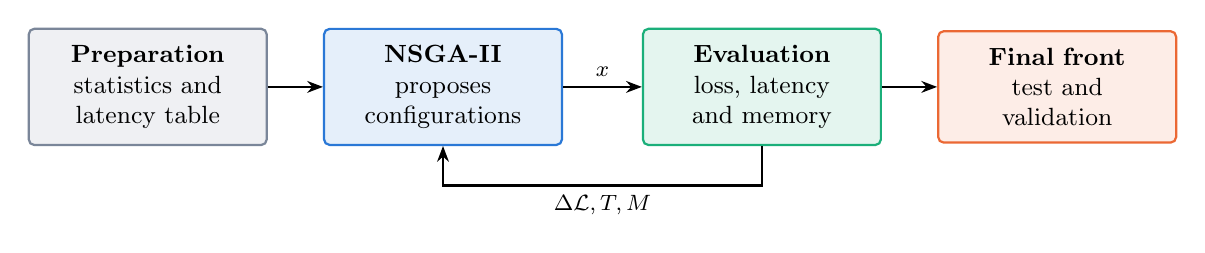
\begin{tikzpicture}[
  box/.style={draw, line width=0.8pt, rounded corners=2pt, align=center, font=\small, text width=2.6cm,
              inner sep=6pt, minimum height=1.4cm},
  arr/.style={-{Stealth[length=2mm]}, thick},
  lab/.style={font=\footnotesize},
  node distance=7mm]
\node[box, draw=cprep, fill=cprep!12] (prep) {\textbf{Preparation}\\statistics and\\latency table};
\node[box, draw=csearch, fill=csearch!12, right=of prep] (nsga) {\textbf{NSGA-II}\\proposes\\configurations};
\node[box, draw=ceval, fill=ceval!12, right=10mm of nsga] (eval) {\textbf{Evaluation}\\loss, latency\\and memory};
\node[box, draw=cfinal, fill=cfinal!12, right=of eval] (final) {\textbf{Final front}\\test and\\validation};
\draw[arr] (prep) -- (nsga);
\draw[arr] (nsga) -- node[lab, above] {$x$} (eval);
\draw[arr] (eval.south) -- ++(0,-0.5) -| node[lab, pos=0.25, below] {$\dloss, T, M$} (nsga.south);
\draw[arr] (eval) -- (final);
\end{tikzpicture}
\end{adjustbox}
\caption{Pipeline of the hardware-aware search. Before the search, the activation statistics, the
sublayer removal ranking and the latency table of the GPU are computed once. NSGA-II proposes
configurations $x$; each is evaluated by its calibration loss $\dloss$ and its predicted latency $T$ and
memory $M$. The final front is scored on test sets and validated with deployed models.}\label{fig:pipeline}
\end{figure}
\end{frame}

\begin{frame}{Experiments on Qwen2.5-0.5B-Instruct}{The fronts}
\begin{figure}
\centering
\begin{adjustbox}{minipage=\linewidth, max width=\linewidth, max totalheight=0.76\textheight, center}
\centering
\begin{subfigure}{0.49\linewidth}
  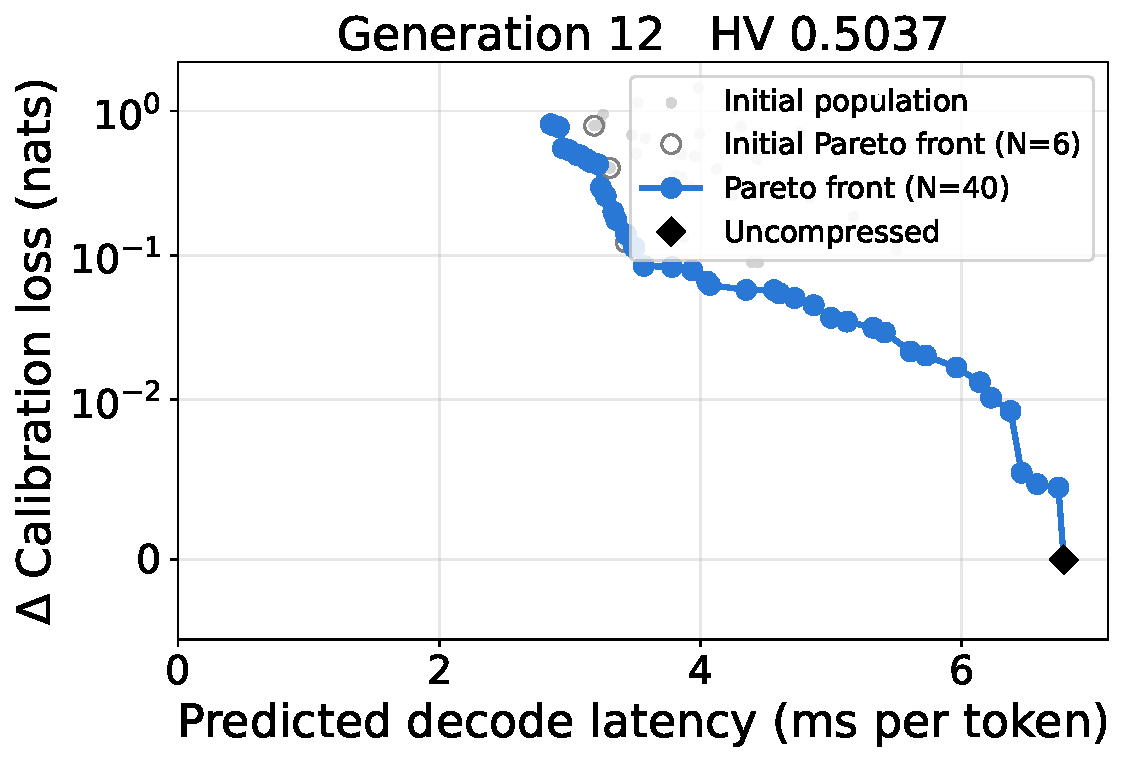
\includegraphics[width=\linewidth]{figures/front_2obj_with_init_pop_log.pdf}
  \caption{Log scale.}
\end{subfigure}\hfill
\begin{subfigure}{0.49\linewidth}
  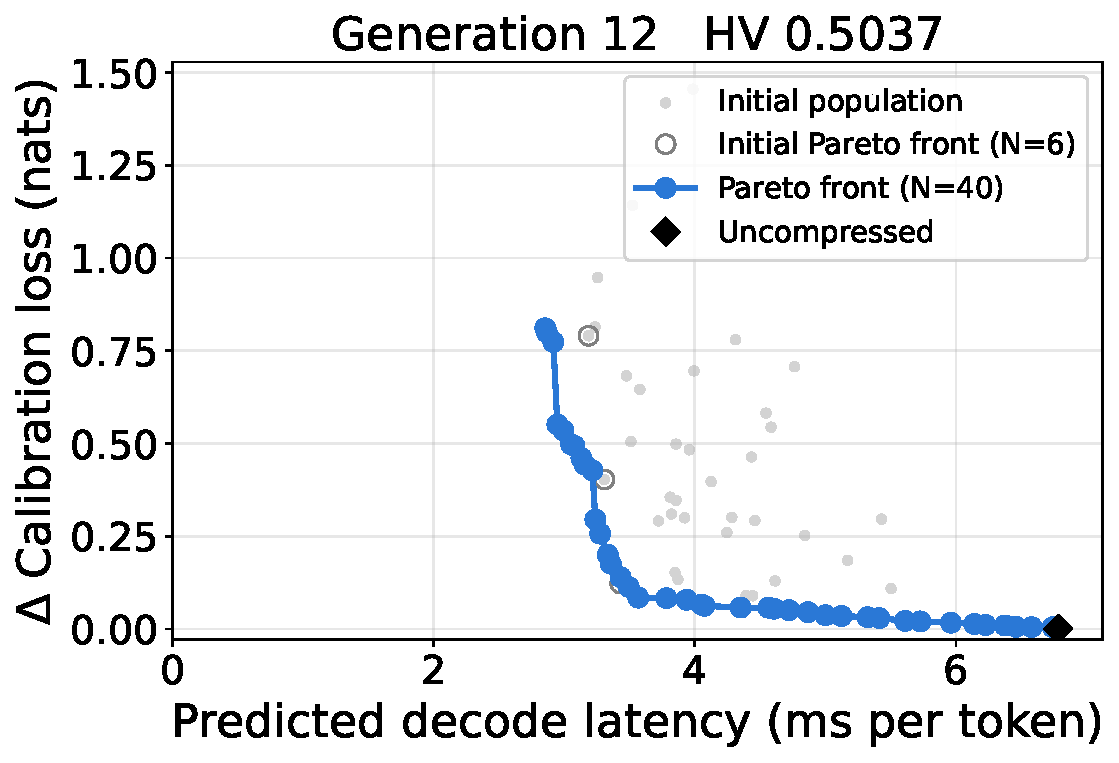
\includegraphics[width=\linewidth]{figures/front_2obj_with_init_pop_linear.pdf}
  \caption{Linear scale.}
\end{subfigure}
\end{adjustbox}
\caption{Two-objective search: initial population (grey), initial front (hollow) and final front after
12 generations, with the loss on a log scale (linear below 0.01 nats) and on a linear scale.}\label{fig:front2}
\end{figure}
\end{frame}

\begin{frame}{Experiments on Qwen2.5-0.5B-Instruct}{The fronts}
\begin{figure}
\centering
\begin{adjustbox}{minipage=\linewidth, max width=\linewidth, max totalheight=0.76\textheight, center}
\centering
\begin{subfigure}{0.49\linewidth}
  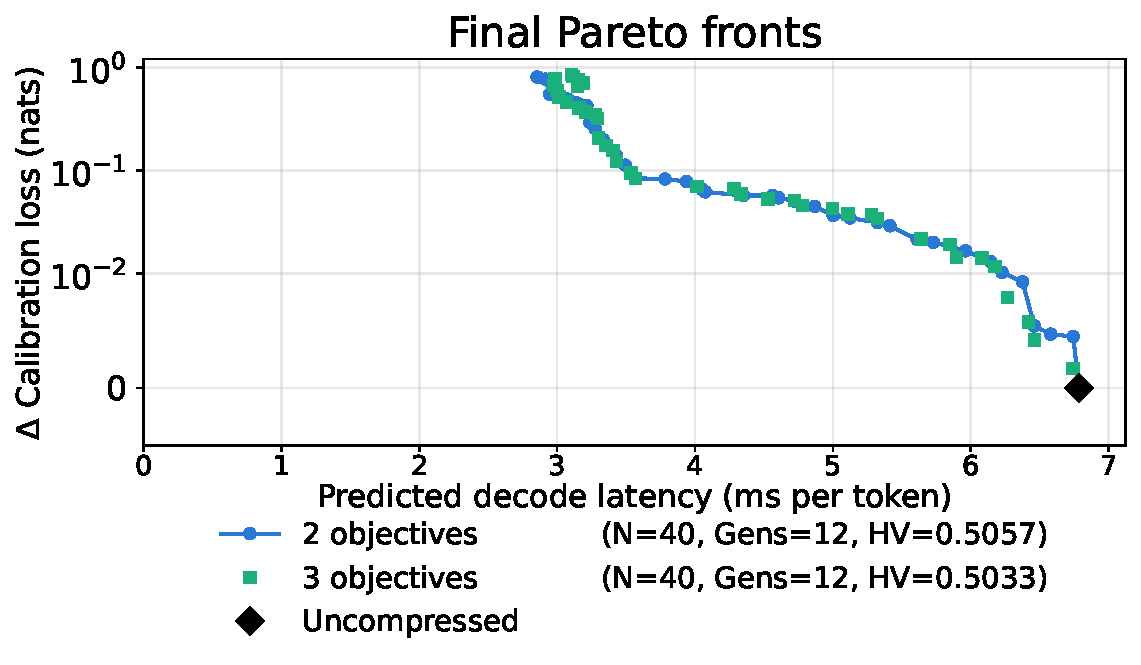
\includegraphics[width=\linewidth]{figures/fronts_latency_log.pdf}
  \caption{Latency, log scale.}
\end{subfigure}\hfill
\begin{subfigure}{0.49\linewidth}
  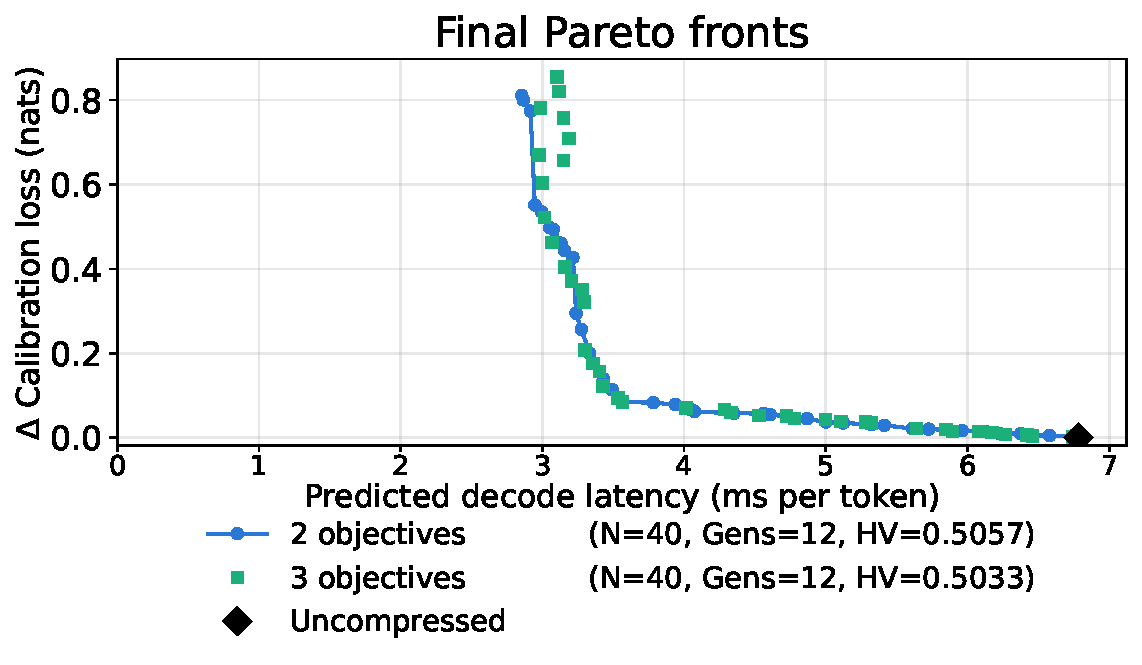
\includegraphics[width=\linewidth]{figures/fronts_latency_linear.pdf}
  \caption{Latency, linear scale.}
\end{subfigure}\\[6pt]
\begin{subfigure}{0.49\linewidth}
  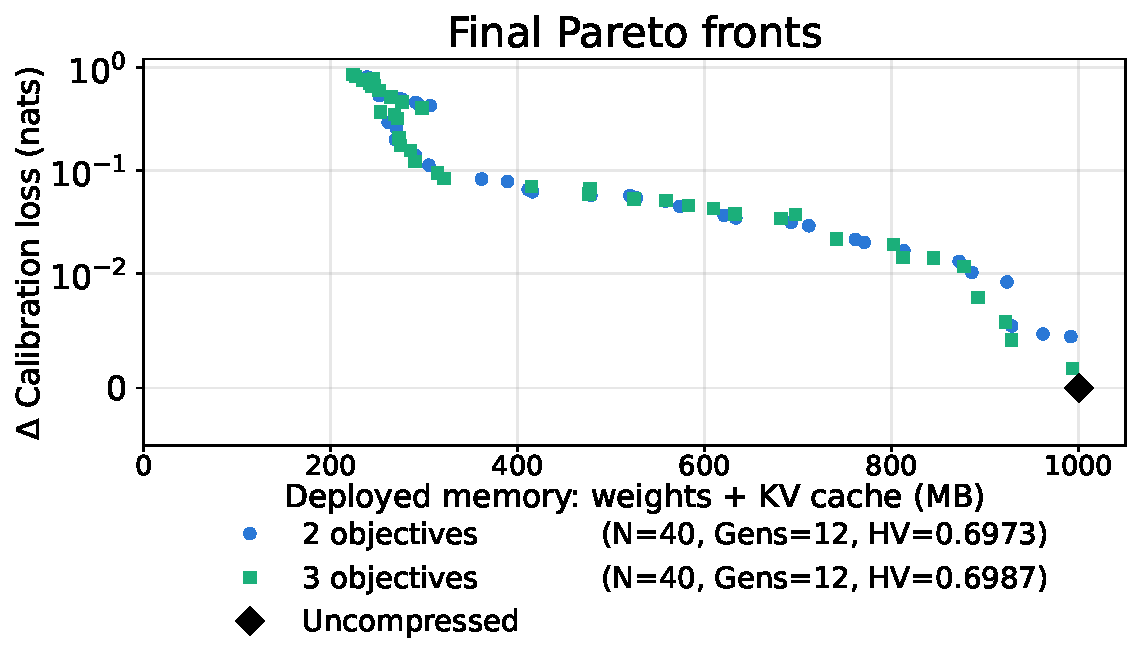
\includegraphics[width=\linewidth]{figures/fronts_memory_log.pdf}
  \caption{Memory, log scale.}
\end{subfigure}\hfill
\begin{subfigure}{0.49\linewidth}
  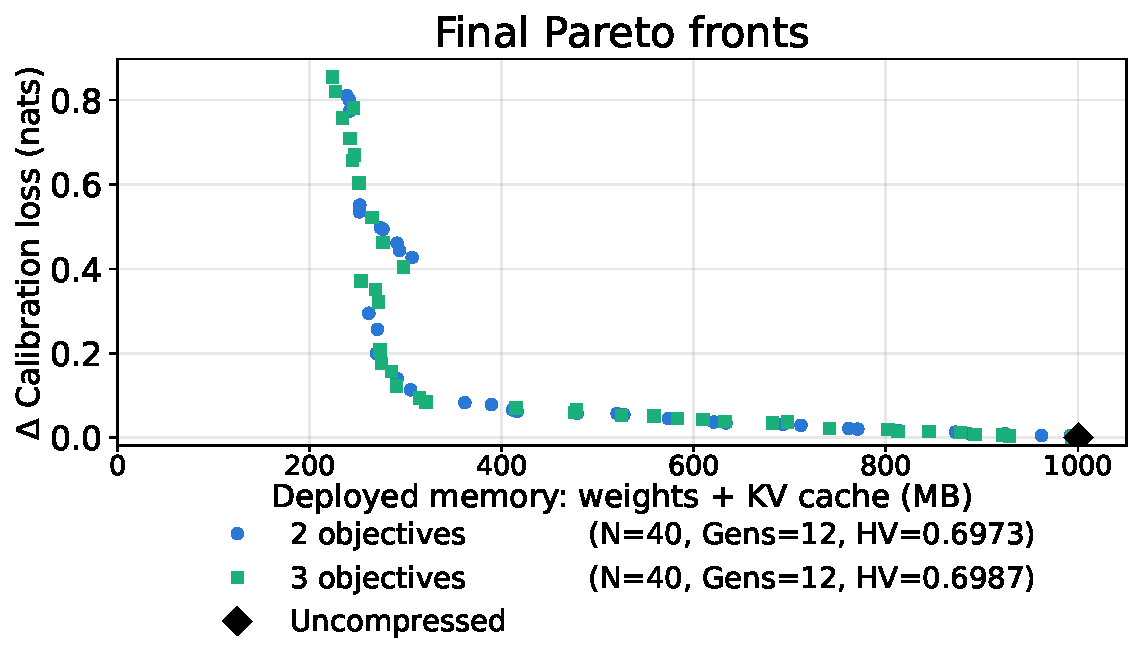
\includegraphics[width=\linewidth]{figures/fronts_memory_linear.pdf}
  \caption{Memory, linear scale.}
\end{subfigure}
\end{adjustbox}
\caption{Final fronts of the two searches: loss against predicted decode latency (top) and against
deployed memory (bottom), on a log scale (linear below 0.01 nats, left) and a linear scale (right). A
front is drawn as a line only in the objectives it optimized; elsewhere its points are not ordered
along the axis.}\label{fig:fronts}
\end{figure}
\end{frame}

\begin{frame}{Experiments on Qwen2.5-0.5B-Instruct}{Test perplexity}
\begin{table}
\centering
\begin{adjustbox}{width=\linewidth, totalheight=0.64\textheight, keepaspectratio, center}
\centering
\small
\begin{tabular}{lcccccc}
\toprule
Search & Latency (ms) & Memory (MB) & Bits/weight & $\dloss$ (nats) & WikiText-2 & C4 \\
\midrule
Uncompressed & 6.78 (1.00$\times$) & 1001 & 16.00 & 0 & 14.33 & 22.33 \\
\midrule
2 obj.  & 5.73 (1.18$\times$) & 771  & 12.28 & 0.020 & 14.67 & 22.80 \\
        & 4.61 (1.47$\times$) & 527  & 8.34  & 0.054 & 15.00 & 23.55 \\
        & 3.57 (1.90$\times$) & 321  & 5.00  & 0.084 & 15.73 & 24.29 \\
        & 3.16 (2.15$\times$) & 294  & 4.60  & 0.443 & 25.57 & 35.59 \\
        & 2.85 (2.38$\times$) & 239  & 3.72  & 0.811 & 39.12 & 51.80 \\
\midrule
3 obj.  & 5.85 (1.16$\times$) & 802  & 12.79 & 0.019 & 14.56 & 22.83 \\
        & 4.53 (1.50$\times$) & 525  & 8.29  & 0.053 & 15.40 & 23.42 \\
        & 3.40 (1.99$\times$) & 286  & 4.42  & 0.157 & 17.18 & 26.78 \\
        & 3.15 (2.15$\times$) & 234  & 3.59  & 0.757 & 44.46 & 54.86 \\
        & 2.98 (2.28$\times$) & 247  & 3.84  & 0.670 & 32.87 & 49.46 \\
\bottomrule
\end{tabular}
\end{adjustbox}
\caption{Test perplexity (32 windows of 2048 tokens each) of the uncompressed model and of points of the
final fronts of the two searches. In parentheses: the speedup over the uncompressed model (6.78\,ms).}\label{tab:test}
\end{table}
\end{frame}

\begin{frame}{Experiments on Qwen2.5-0.5B-Instruct}{Test perplexity}
\begin{figure}
\centering
\begin{adjustbox}{minipage=\linewidth, max width=\linewidth, max totalheight=0.76\textheight, center}
\centering
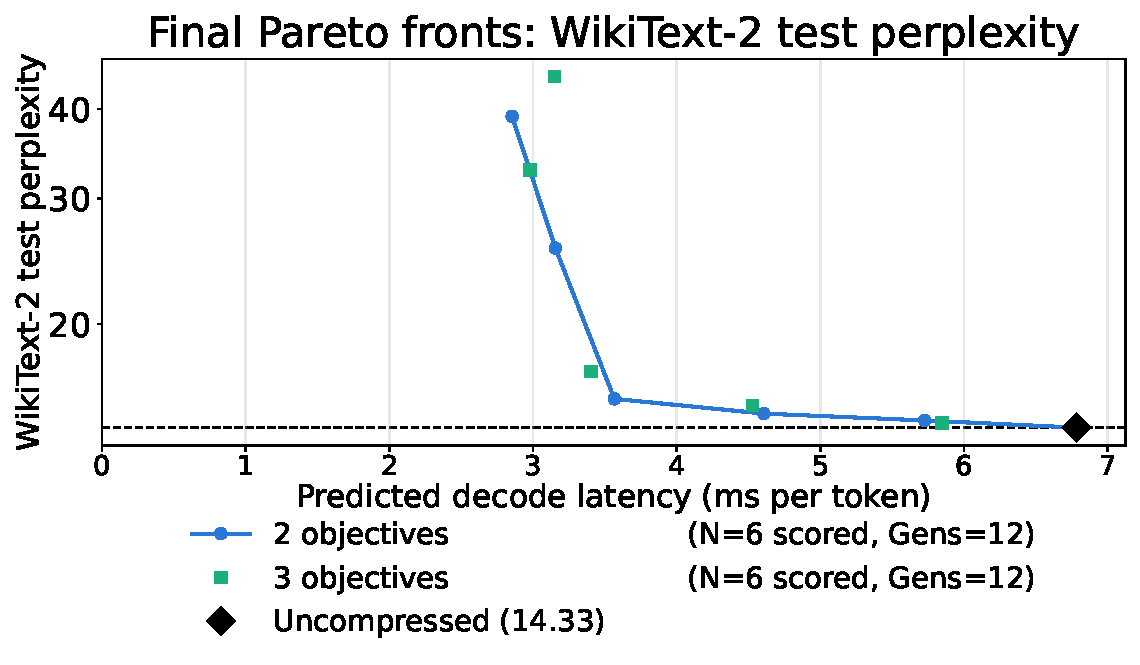
\includegraphics[width=0.62\linewidth]{figures/test_wikitext2_latency.pdf}
\end{adjustbox}
\caption{WikiText-2 test perplexity of the scored points against predicted decode latency.}\label{fig:test}
\end{figure}
\end{frame}

\begin{frame}{Experiments on Qwen2.5-0.5B-Instruct}{Two objectives against three}
\begin{table}
\centering
\begin{adjustbox}{width=\linewidth, totalheight=0.64\textheight, keepaspectratio, center}
\centering
\small
\begin{tabular}{rcccccc}
\toprule
Objectives & \multicolumn{2}{c}{\{loss, latency, memory\}} & \multicolumn{2}{c}{\{loss, latency\}} & \multicolumn{2}{c}{\{loss, memory\}} \\
\cmidrule(lr){2-3}\cmidrule(lr){4-5}\cmidrule(lr){6-7}
Generation & 2 obj. & 3 obj. & 2 obj. & 3 obj. & 2 obj. & 3 obj. \\
\midrule
1  & 0.3302          & 0.3302 & 0.4550          & 0.4550 & 0.6504          & 0.6504 \\
2  & \textbf{0.3335} & 0.3313 & \textbf{0.4654} & 0.4587 & \textbf{0.6650} & 0.6555 \\
3  & \textbf{0.3375} & 0.3333 & \textbf{0.4676} & 0.4668 & \textbf{0.6696} & 0.6671 \\
4  & \textbf{0.3444} & 0.3398 & \textbf{0.4786} & 0.4755 & \textbf{0.6815} & 0.6691 \\
5  & \textbf{0.3500} & 0.3461 & \textbf{0.4877} & 0.4836 & \textbf{0.6833} & 0.6757 \\
6  & \textbf{0.3511} & 0.3492 & \textbf{0.4893} & 0.4876 & \textbf{0.6837} & 0.6788 \\
7  & \textbf{0.3584} & 0.3539 & \textbf{0.4967} & 0.4941 & \textbf{0.6892} & 0.6845 \\
8  & \textbf{0.3622} & 0.3564 & \textbf{0.5000} & 0.4974 & \textbf{0.6942} & 0.6870 \\
9  & \textbf{0.3638} & 0.3611 & \textbf{0.5025} & 0.4998 & \textbf{0.6946} & 0.6939 \\
10 & \textbf{0.3651} & 0.3633 & \textbf{0.5050} & 0.5020 & \textbf{0.6961} & 0.6960 \\
11 & \textbf{0.3655} & 0.3639 & \textbf{0.5056} & 0.5026 & 0.6971          & \textbf{0.6974} \\
12 & \textbf{0.3655} & 0.3646 & \textbf{0.5057} & 0.5033 & 0.6973          & \textbf{0.6987} \\
\bottomrule
\end{tabular}
\end{adjustbox}
\caption{Hypervolume of each generation's front with one shared normalization, in all three objectives
and in the two projections. Generation 1 is identical because both searches start from the same
population.}\label{tab:hv}
\end{table}
\end{frame}

\begin{frame}{Experiments on Qwen2.5-0.5B-Instruct}{Two objectives against three}
\begin{figure}
\centering
\begin{adjustbox}{minipage=\linewidth, max width=\linewidth, max totalheight=0.76\textheight, center}
\centering
\begin{subfigure}{0.72\linewidth}
  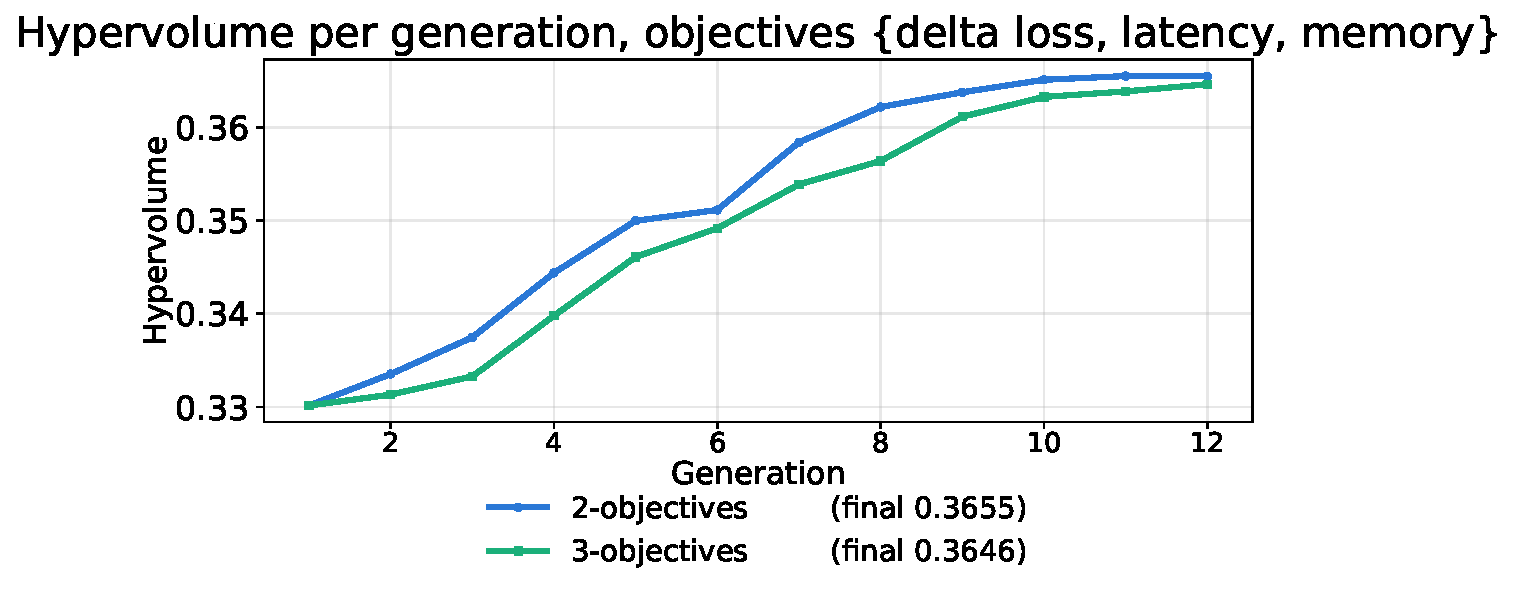
\includegraphics[width=\linewidth]{figures/hv_3d.pdf}
  \caption{\{loss, latency, memory\}.}
\end{subfigure}\\[6pt]
\begin{subfigure}{0.49\linewidth}
  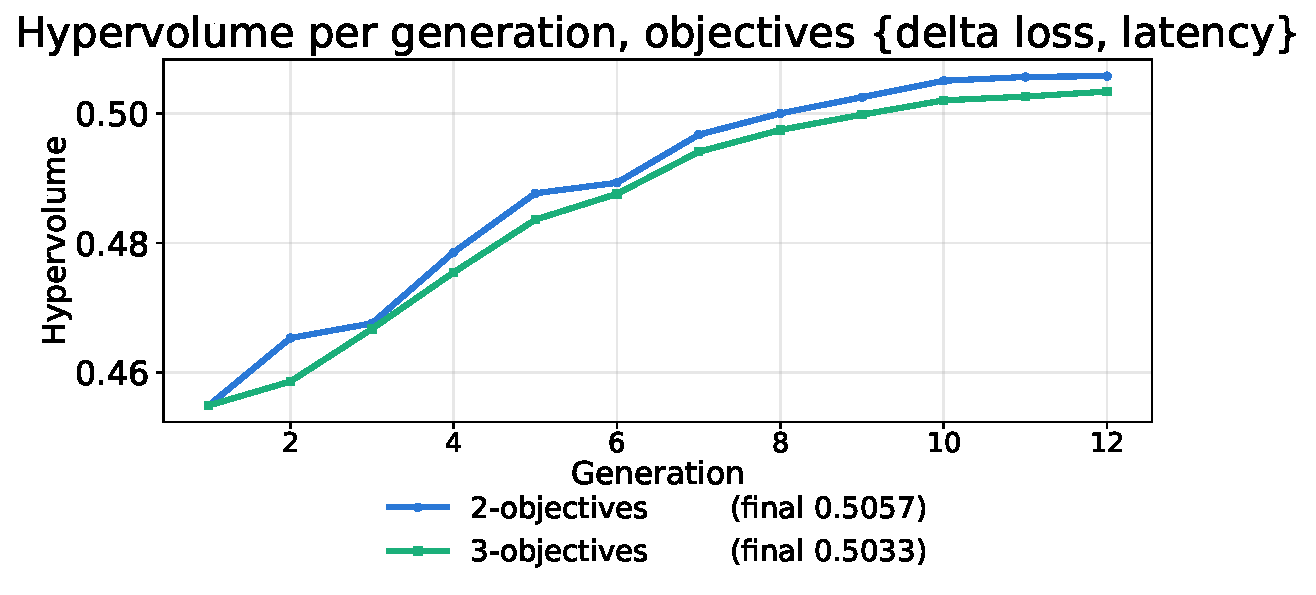
\includegraphics[width=\linewidth]{figures/hv_latency.pdf}
  \caption{\{loss, latency\}.}
\end{subfigure}\hfill
\begin{subfigure}{0.49\linewidth}
  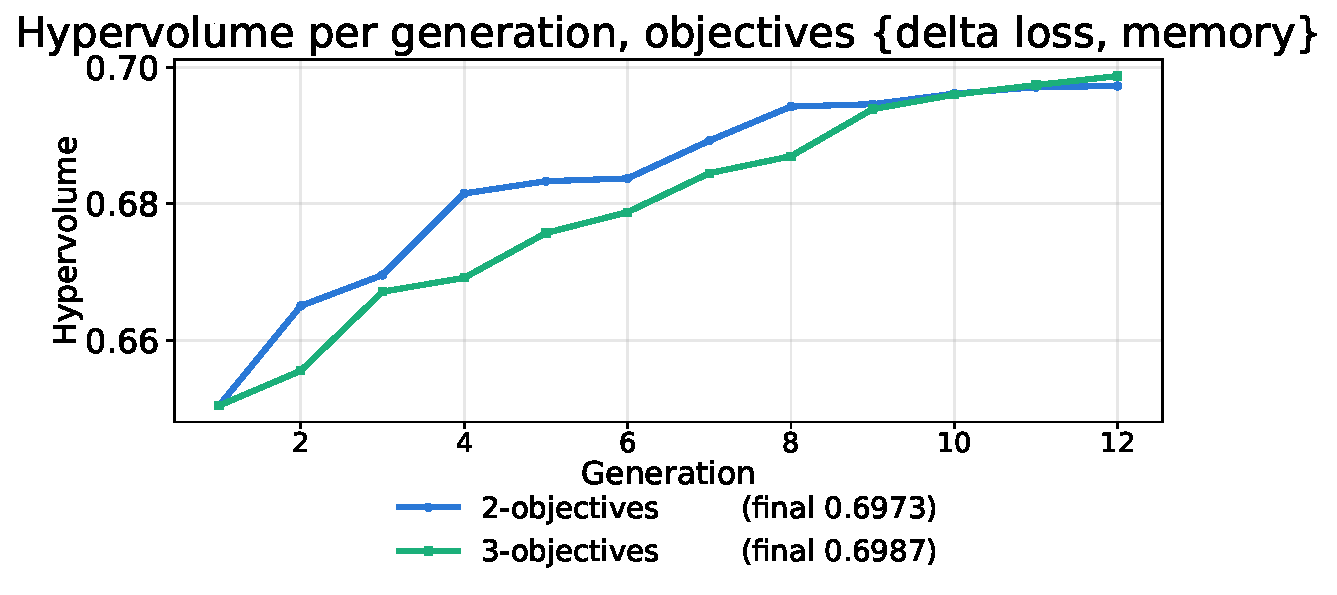
\includegraphics[width=\linewidth]{figures/hv_memory.pdf}
  \caption{\{loss, memory\}.}
\end{subfigure}
\end{adjustbox}
\caption{Hypervolume per generation of the two searches with one shared normalization: in all three
objectives (a), and in the projections \{loss, latency\} (b) and \{loss, memory\} (c).}\label{fig:hv}
\end{figure}
\end{frame}

\begin{frame}{Experiments on Qwen2.5-0.5B-Instruct}{Two objectives against three}
\begin{figure}
\centering
\begin{adjustbox}{minipage=\linewidth, max width=\linewidth, max totalheight=0.76\textheight, center}
\centering
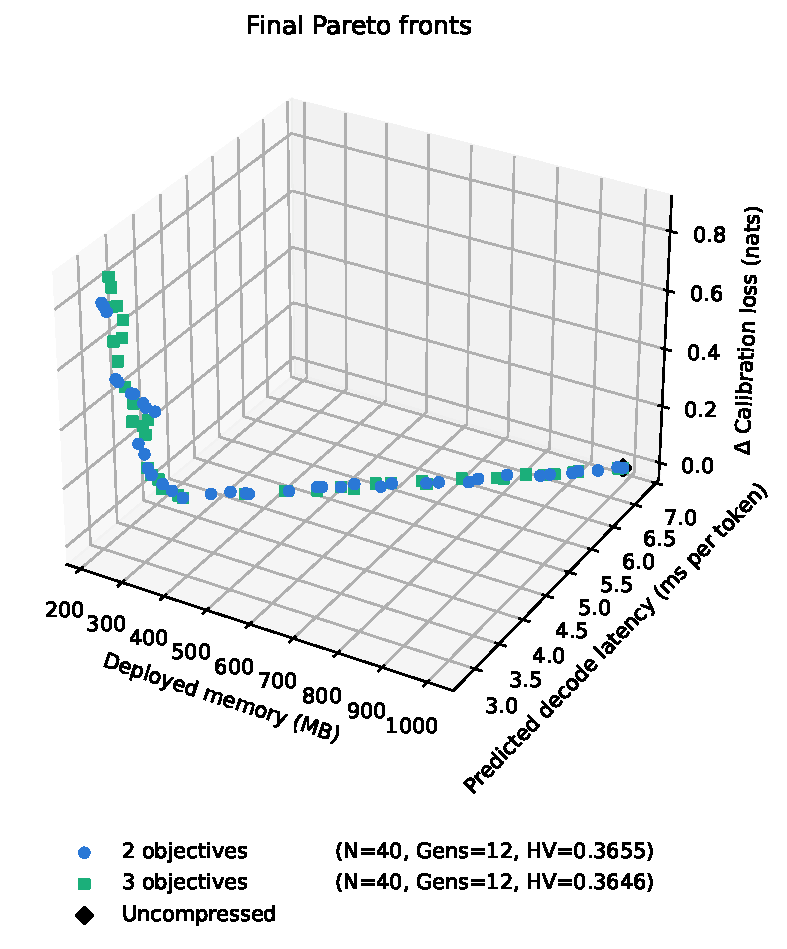
\includegraphics[width=0.66\linewidth]{figures/fronts_3d.pdf}
\end{adjustbox}
\caption{Final fronts of both searches in all three objectives. Both lie along a thin curve because
memory and latency decrease together on this model.}\label{fig:fronts3d}
\end{figure}
\end{frame}

\begin{frame}{A100, three objectives}{Anatomy of a decode step on the A100}
\begin{table}
\centering
\begin{adjustbox}{width=\linewidth, totalheight=0.64\textheight, keepaspectratio, center}
\centering
\small
\begin{tabular}{lcccc}
\toprule
& \multicolumn{2}{c}{bf16} & \multicolumn{2}{c}{int4, group 128} \\
\cmidrule(lr){2-3}\cmidrule(lr){4-5}
Part of the step & \us & share & \us & share \\
\midrule
MLP products (gate, up, down) $\times24$          & 719  & 18\% & 425  & 12\% \\
Attention products ($q,k,v,o$) $\times24$          & 520  & 13\% & 354  & 10\% \\
Attention over 1024 cached tokens $\times24$       & 301  & 8\%  & 301  & 9\%  \\
Output head ($151936\times896$)                    & 163  & 4\%  & 82   & 2\%  \\
Norms, rotary, activations, residuals $\times24$   & 921  & 23\% & 921  & 27\% \\
Fixed (embedding, final norm, logits)              & 1324 & 34\% & 1324 & 39\% \\
\midrule
Total                                              & 3947 &      & 3407 &      \\
\bottomrule
\end{tabular}
\end{adjustbox}
\caption{Predicted GPU time of one decode step of Qwen2.5-0.5B-Instruct (batch 1, 1024 tokens of
context) on the A100.}\label{tab:anatomy-a100}
\end{table}
\end{frame}

\begin{frame}{A100, three objectives}{The front}
\begin{figure}
\centering
\begin{adjustbox}{minipage=\linewidth, max width=\linewidth, max totalheight=0.76\textheight, center}
\centering
\begin{subfigure}{0.49\linewidth}
  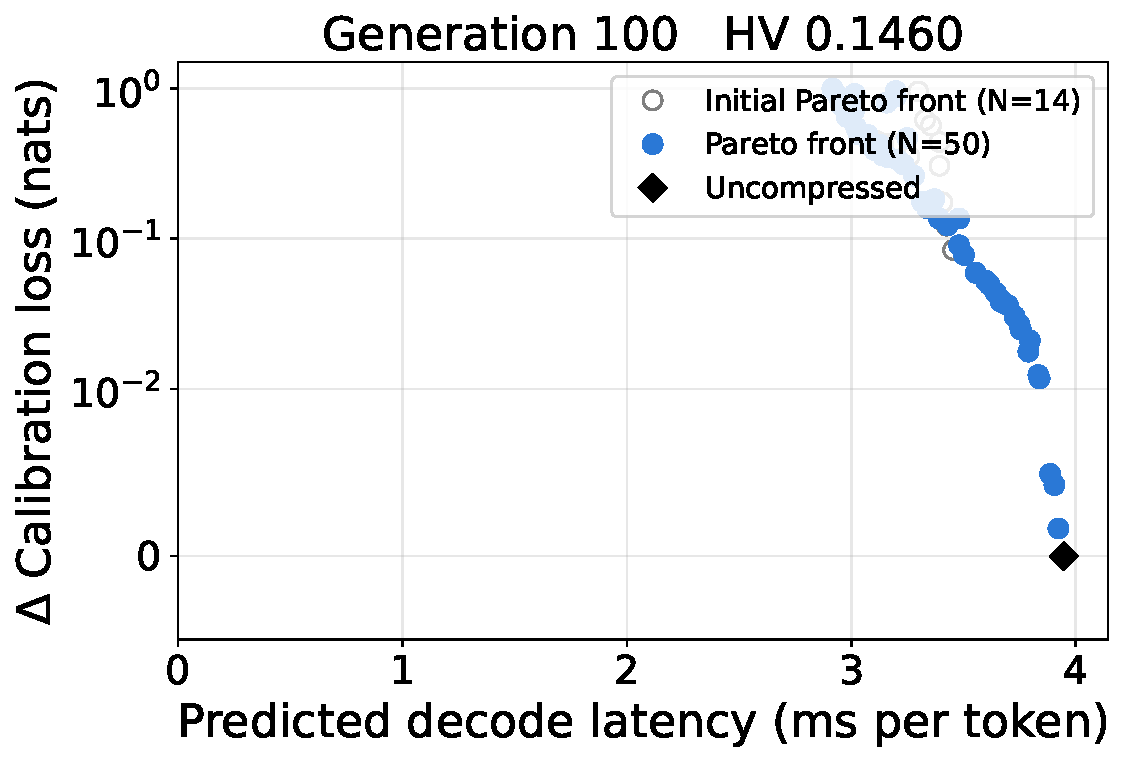
\includegraphics[width=\linewidth]{figures/a100_3obj_front_latency.pdf}
  \caption{Against predicted decode latency.}
\end{subfigure}\hfill
\begin{subfigure}{0.49\linewidth}
  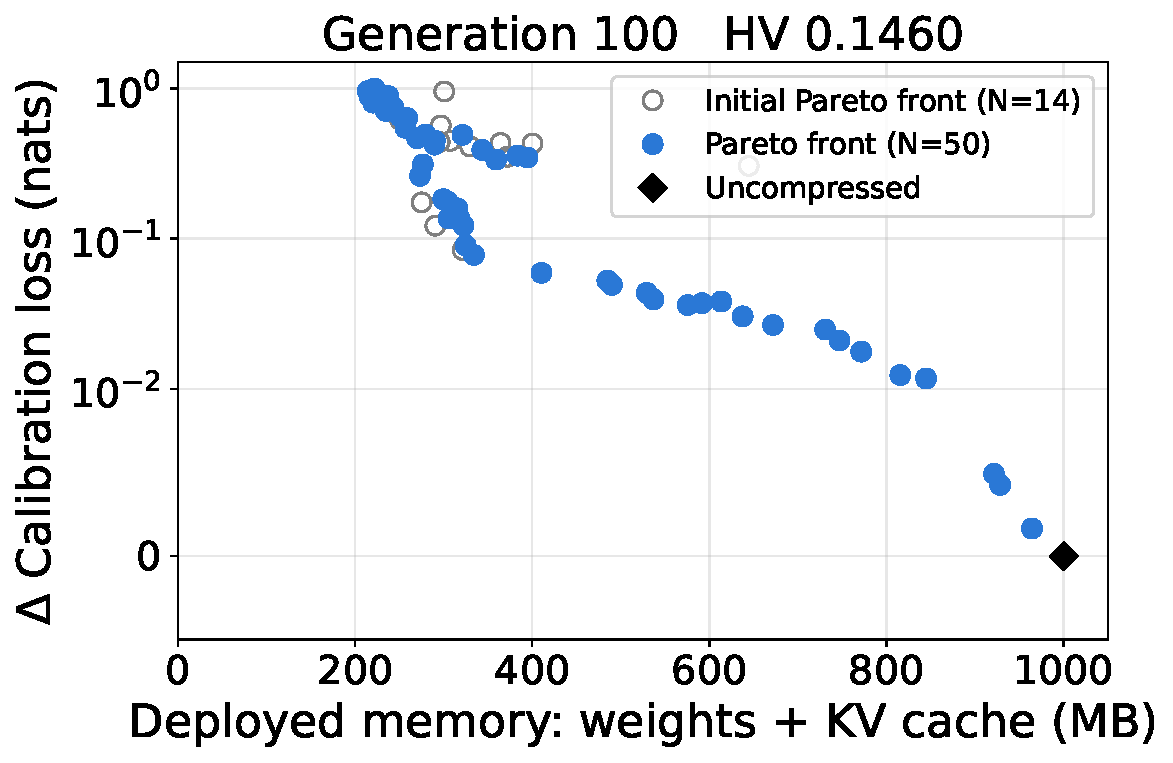
\includegraphics[width=\linewidth]{figures/a100_3obj_front_memory.pdf}
  \caption{Against deployed memory.}
\end{subfigure}
\end{adjustbox}
\caption{Three-objective search on the A100: final front (50 solutions), initial front and the
uncompressed model.}\label{fig:a100-3obj-front}
\end{figure}
\end{frame}

\begin{frame}{A100, three objectives}{Test perplexity}
\begin{table}
\centering
\begin{adjustbox}{width=\linewidth, totalheight=0.64\textheight, keepaspectratio, center}
\centering
\footnotesize
\setlength{\tabcolsep}{3pt}
\begin{tabular}{lccccc}
\toprule
Configuration & Latency (ms) & Memory (MB) & $\dloss$ (nats) & WikiText-2 & C4 \\
\midrule
uncompressed & 3.95 (1.00$\times$) & 1001 & 0 & 14.34 & 22.33 \\
\midrule
int4 in up and part of down & 3.73 (1.06$\times$) & 638 & 0.030 & 14.64 & 23.08 \\
mostly int4 & 3.48 (1.14$\times$) & 325 & 0.091 & 15.92 & 24.65 \\
int4, MLP pruned in 2 bands, $-3$ attn & 3.23 (1.22$\times$) & 277 & 0.312 & 21.37 & 32.11 \\
mostly int4, MLP 5/8 in 1 band, $-6$ attn & 3.07 (1.29$\times$) & 321 & 0.492 & 27.93 & 38.47 \\
int4, MLP pruned in 2 bands, $-6$ attn, $-4$ MLP & 2.92 (1.35$\times$) & 222 & 0.998 & 60.31 & 69.15 \\
\bottomrule
\end{tabular}
\end{adjustbox}
\caption{Test perplexity (32 windows of 2048 tokens each) of the uncompressed model and of points of the
final three-objective front. In parentheses: the speedup over the uncompressed model (3.95\,ms).}\label{tab:a100-3obj-test}
\end{table}
\end{frame}

\begin{frame}{A100, three objectives}{Test perplexity}
\begin{figure}
\centering
\begin{adjustbox}{minipage=\linewidth, max width=\linewidth, max totalheight=0.76\textheight, center}
\centering
\begin{subfigure}{0.49\linewidth}
  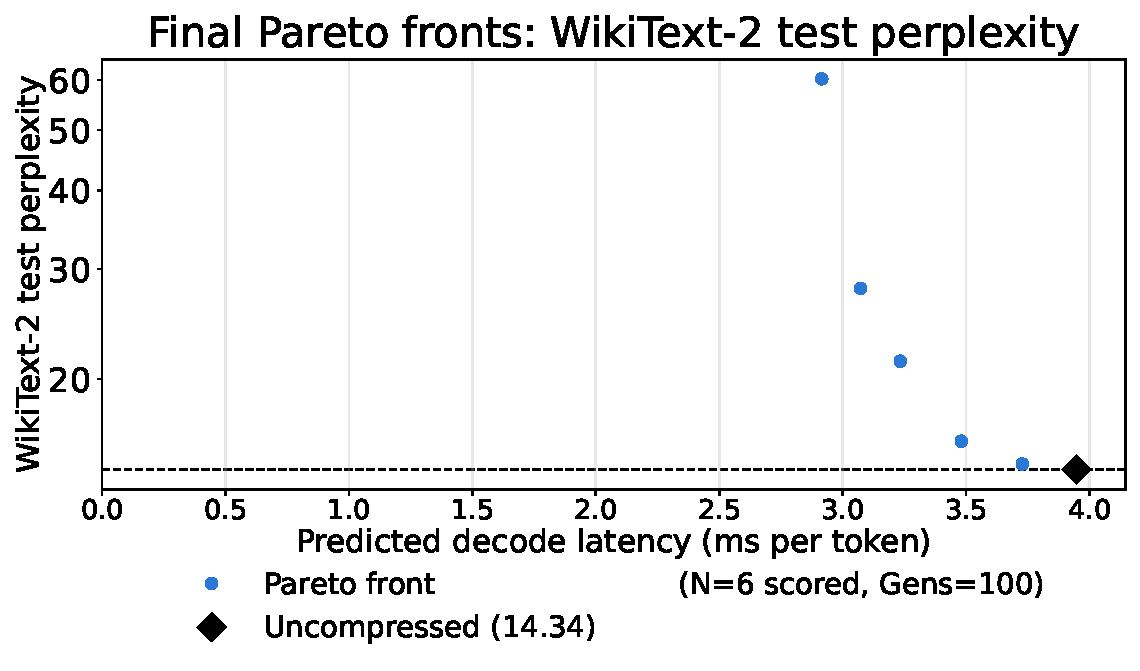
\includegraphics[width=\linewidth]{figures/a100_3obj_test_wikitext2.pdf}
  \caption{WikiText-2 test.}
\end{subfigure}\hfill
\begin{subfigure}{0.49\linewidth}
  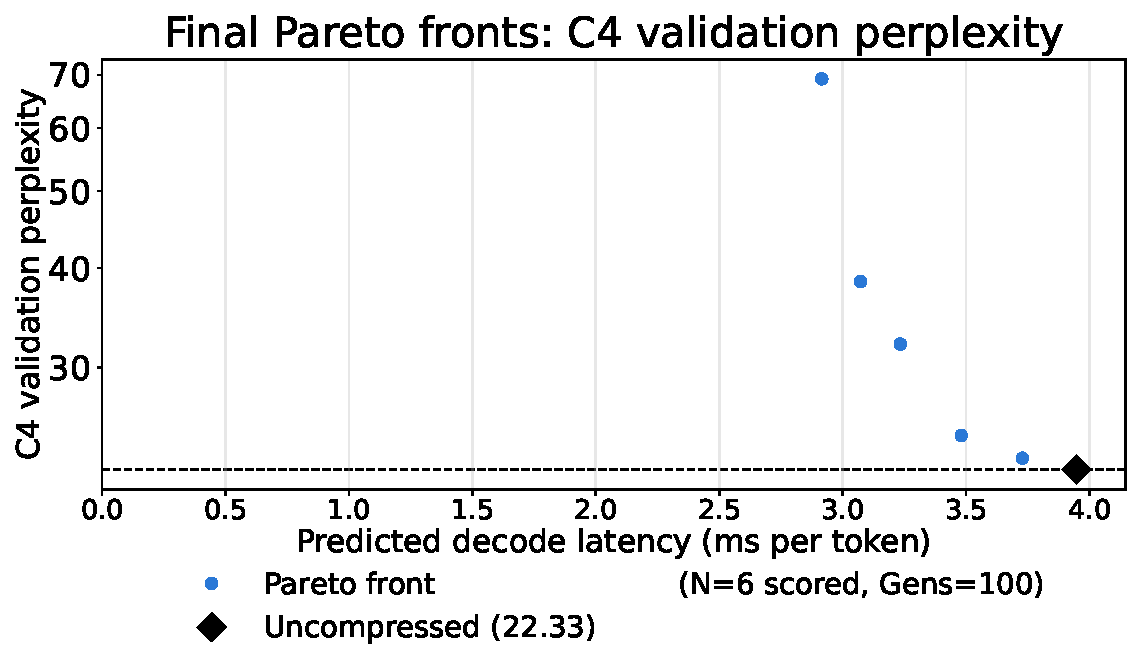
\includegraphics[width=\linewidth]{figures/a100_3obj_test_c4.pdf}
  \caption{C4 validation.}
\end{subfigure}
\end{adjustbox}
\caption{Test perplexity of the scored points of the three-objective search against predicted decode
latency.}\label{fig:a100-3obj-test}
\end{figure}
\end{frame}

\begin{frame}{A100, three objectives}{Validation against the deployed models}
\begin{table}
\centering
\begin{adjustbox}{width=\linewidth, totalheight=0.64\textheight, keepaspectratio, center}
\centering
\footnotesize
\setlength{\tabcolsep}{4pt}
\begin{tabular}{lcccccccc}
\toprule
& \multicolumn{3}{c}{GPU time (ms)} & Eager & \multicolumn{2}{c}{Loss (nats)} & \multicolumn{2}{c}{Speedup} \\
\cmidrule(lr){2-4}\cmidrule(lr){6-7}\cmidrule(lr){8-9}
Configuration & pred. & meas. & error & (ms) & sim. & deployed & GPU & eager \\
\midrule
int4, MLP pruned in 2 bands, $-6$ attn, $-4$ MLP  & 2.83 & 2.90 & $-2.7\%$ & 10.81 & 3.9098 & 3.9119 & 1.32 & 1.06 \\
mostly int4, MLP 5/8 in 1 band, $-6$ attn  & 2.98 & 3.05 & $-2.1\%$ & 11.21 & 3.4023 & 3.4052 & 1.26 & 1.02 \\
int4, MLP pruned in 2 bands, $-3$ attn            & 3.13 & 3.17 & $-1.4\%$ & 11.99 & 3.1785 & 3.1786 & 1.21 & 0.95 \\
mostly int4                                       & 3.36 & 3.44 & $-2.3\%$ & 12.37 & 2.9839 & 2.9832 & 1.11 & 0.92 \\
bf16 attention and head, int4 MLP                 & 3.61 & 3.63 & $-0.6\%$ & 12.04 & 2.9206 & 2.9202 & 1.05 & 0.95 \\
uncompressed                                      & 3.83 & 3.87 & $-1.1\%$ & 11.39 & 2.8916 & 2.8916 & 0.99 & 1.00 \\
\bottomrule
\end{tabular}
\end{adjustbox}
\caption{Three-objective search: predicted against measured GPU time of the deployed models (one token,
batch 1), eager wall-clock time, calibration loss on two windows, and the measured speedup over a
separately timed uncompressed reference (3.83\,ms, 11.41\,ms eager).}\label{tab:a100-3obj-validation}
\end{table}
\end{frame}

\begin{frame}{A100, two objectives}{The front}
\begin{figure}
\centering
\begin{adjustbox}{minipage=\linewidth, max width=\linewidth, max totalheight=0.76\textheight, center}
\centering
\begin{subfigure}{0.49\linewidth}
  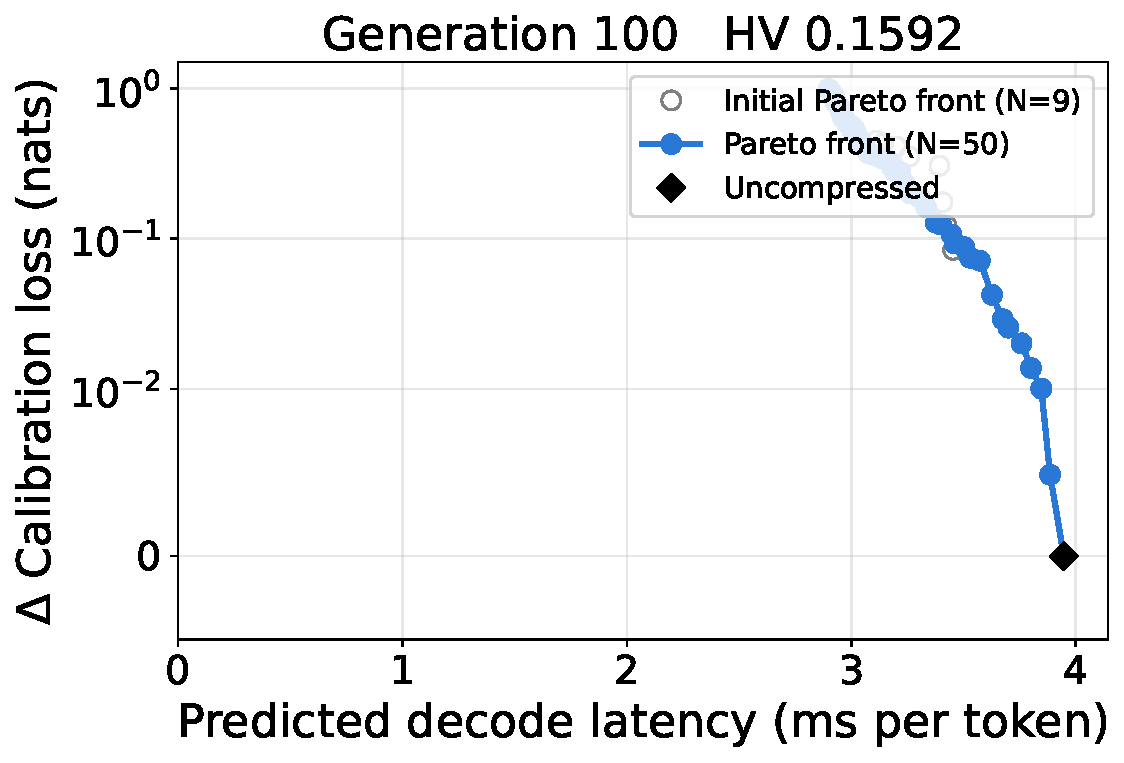
\includegraphics[width=\linewidth]{figures/a100_2obj_front_latency.pdf}
  \caption{Against predicted decode latency (objective).}
\end{subfigure}\hfill
\begin{subfigure}{0.49\linewidth}
  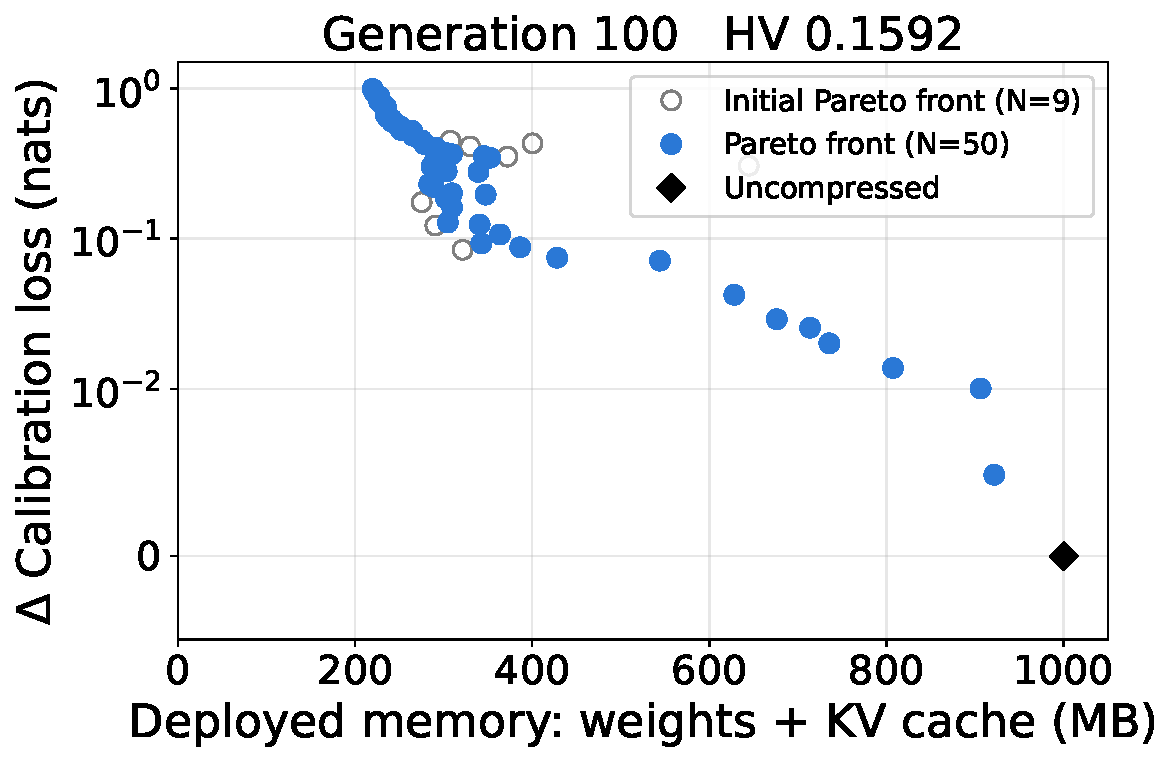
\includegraphics[width=\linewidth]{figures/a100_2obj_front_memory.pdf}
  \caption{Against deployed memory (reported).}
\end{subfigure}
\end{adjustbox}
\caption{Two-objective search on the A100: final front (50 solutions), initial front and the uncompressed
model.}\label{fig:a100-2obj-front}
\end{figure}
\end{frame}

\begin{frame}{A100, two objectives}{The front}
\begin{table}
\centering
\begin{adjustbox}{width=\linewidth, totalheight=0.64\textheight, keepaspectratio, center}
\centering
\footnotesize
\setlength{\tabcolsep}{3pt}
\begin{tabular}{lccccc}
\toprule
Configuration & Latency (ms) & Memory (MB) & $\dloss$ (nats) & WikiText-2 & C4 \\
\midrule
uncompressed & 3.95 (1.00$\times$) & 1001 & 0 & 14.34 & 22.33 \\
\midrule
mostly int4 & 3.50 (1.13$\times$) & 387 & 0.088 & 15.65 & 24.21 \\
int4, $-3$ attn & 3.24 (1.22$\times$) & 284 & 0.230 & 18.74 & 28.10 \\
int4, MLP 7/8 in 1 band, $-6$ attn & 3.06 (1.29$\times$) & 291 & 0.402 & 24.65 & 33.99 \\
int4, MLP 5/8 in 2 bands, $-6$ attn, $-1$ MLP & 2.96 (1.33$\times$) & 237 & 0.636 & 33.82 & 46.29 \\
int4, MLP 5/8 in 2 bands, $-6$ attn, $-5$ MLP & 2.90 (1.36$\times$) & 220 & 0.990 & 50.95 & 62.69 \\
\bottomrule
\end{tabular}
\end{adjustbox}
\caption{Test perplexity (32 windows of 2048 tokens each) of the uncompressed model and of points of the
final two-objective front. In parentheses: the speedup over the uncompressed model (3.95\,ms).}\label{tab:a100-2obj-test}
\end{table}
\end{frame}

\begin{frame}{A100, two objectives}{The front}
\begin{figure}
\centering
\begin{adjustbox}{minipage=\linewidth, max width=\linewidth, max totalheight=0.76\textheight, center}
\centering
\begin{subfigure}{0.49\linewidth}
  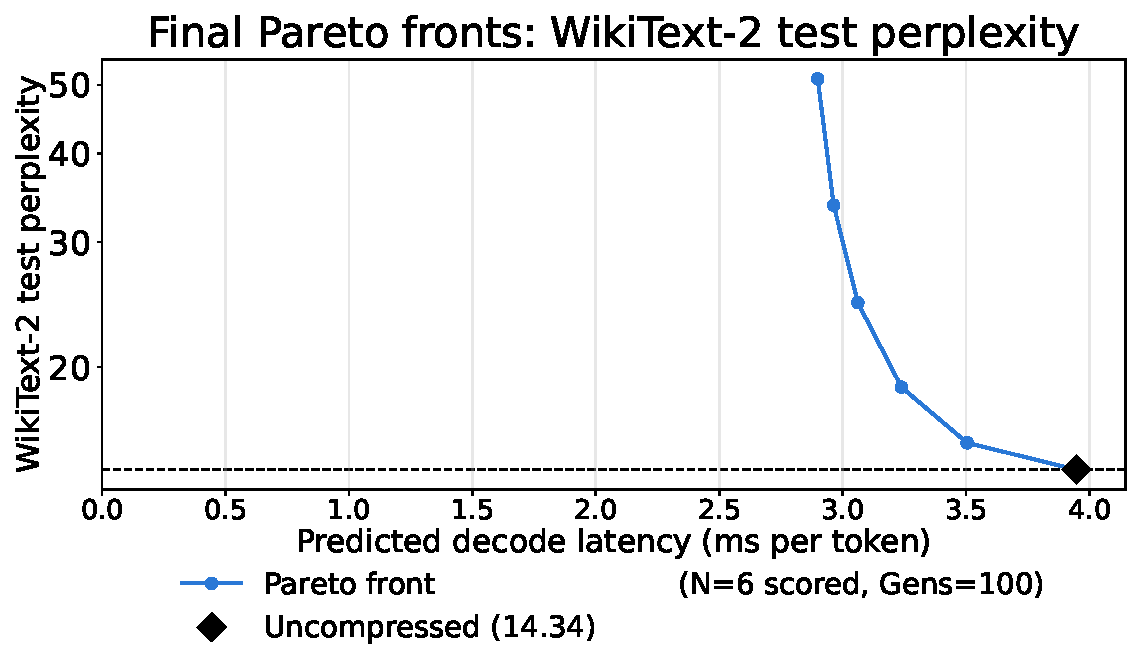
\includegraphics[width=\linewidth]{figures/a100_2obj_test_wikitext2.pdf}
  \caption{WikiText-2 test.}
\end{subfigure}\hfill
\begin{subfigure}{0.49\linewidth}
  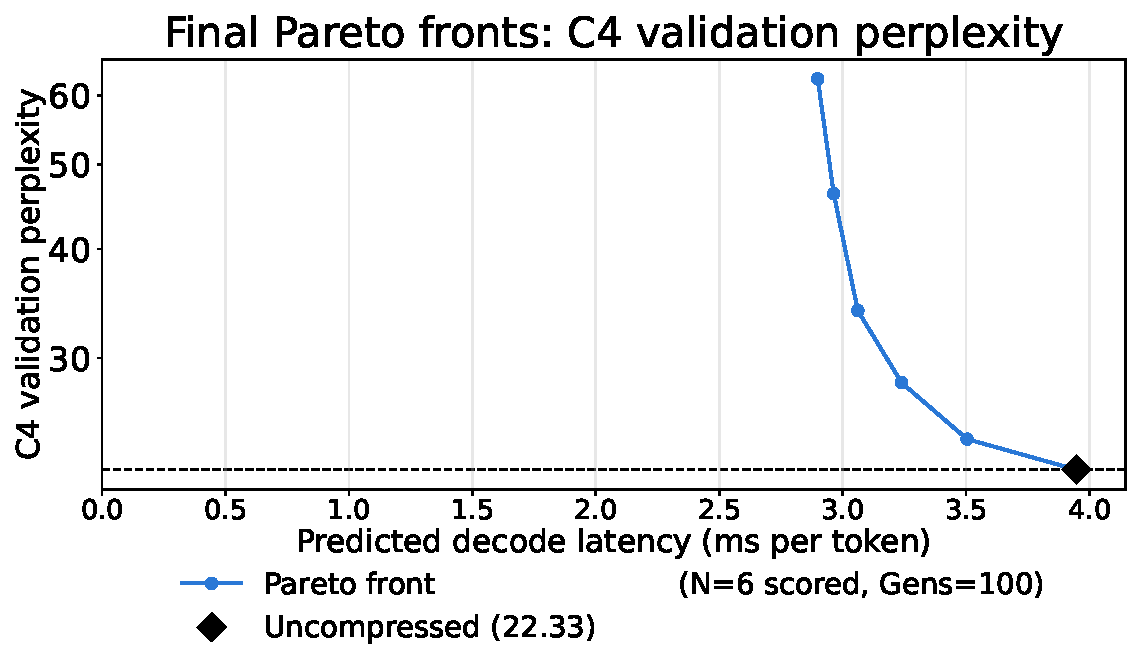
\includegraphics[width=\linewidth]{figures/a100_2obj_test_c4.pdf}
  \caption{C4 validation.}
\end{subfigure}
\end{adjustbox}
\caption{Test perplexity of the scored points of the two-objective search against predicted decode
latency.}\label{fig:a100-2obj-test}
\end{figure}
\end{frame}

\begin{frame}{A100, two objectives}{Validation against the deployed models}
\begin{table}
\centering
\begin{adjustbox}{width=\linewidth, totalheight=0.64\textheight, keepaspectratio, center}
\centering
\footnotesize
\setlength{\tabcolsep}{4pt}
\begin{tabular}{lcccccccc}
\toprule
& \multicolumn{3}{c}{GPU time (ms)} & Eager & \multicolumn{2}{c}{Loss (nats)} & \multicolumn{2}{c}{Speedup} \\
\cmidrule(lr){2-4}\cmidrule(lr){6-7}\cmidrule(lr){8-9}
Configuration & pred. & meas. & error & (ms) & sim. & deployed & GPU & eager \\
\midrule
int4, MLP 5/8 in 2 bands, $-6$ attn, $-5$ MLP & 2.81 & 2.89 & $-2.7\%$ & 11.22 & 3.8935 & 3.8947 & 1.33 & 1.05 \\
int4, MLP 5/8 in 2 bands, $-6$ attn, $-1$ MLP & 2.87 & 2.96 & $-2.9\%$ & 11.53 & 3.5279 & 3.5274 & 1.29 & 1.03 \\
int4, MLP 7/8 in 1 band, $-6$ attn            & 2.97 & 3.00 & $-1.1\%$ & 11.65 & 3.3040 & 3.3042 & 1.28 & 1.02 \\
int4, $-3$ attn                                      & 3.13 & 3.22 & $-2.7\%$ & 12.34 & 3.1046 & 3.1054 & 1.19 & 0.96 \\
mostly int4                                          & 3.38 & 3.44 & $-1.6\%$ & 13.01 & 2.9748 & 2.9747 & 1.11 & 0.91 \\
uncompressed                                         & 3.83 & 3.87 & $-1.0\%$ & 11.89 & 2.8916 & 2.8916 & 0.99 & 1.00 \\
\bottomrule
\end{tabular}
\end{adjustbox}
\caption{Two-objective search: predicted against measured GPU time of the deployed models (one token,
batch 1), eager wall-clock time, calibration loss on two windows, and the measured speedup over a
separately timed uncompressed reference (3.83\,ms, 11.83\,ms eager).}\label{tab:a100-2obj-validation}
\end{table}
\end{frame}

\begin{frame}{A100, two objectives}{Two objectives against three}
\begin{table}
\centering
\begin{adjustbox}{width=\linewidth, totalheight=0.64\textheight, keepaspectratio, center}
\centering
\small
\begin{tabular}{rcccccc}
\toprule
Objectives & \multicolumn{2}{c}{\{loss, latency, memory\}} & \multicolumn{2}{c}{\{loss, latency\}} & \multicolumn{2}{c}{\{loss, memory\}} \\
\cmidrule(lr){2-3}\cmidrule(lr){4-5}\cmidrule(lr){6-7}
Generation & 2 obj. & 3 obj. & 2 obj. & 3 obj. & 2 obj. & 3 obj. \\
\midrule
1   & 0.1202          & \textbf{0.1218} & 0.1686          & 0.1686          & 0.6584          & \textbf{0.6670} \\
5   & 0.1356          & \textbf{0.1381} & 0.1902          & \textbf{0.1906} & 0.6783          & \textbf{0.6938} \\
10  & \textbf{0.1455} & 0.1403          & \textbf{0.2009} & 0.1926          & 0.6960          & \textbf{0.7039} \\
25  & \textbf{0.1497} & 0.1406          & \textbf{0.2051} & 0.1946          & \textbf{0.7004} & 0.6971          \\
50  & \textbf{0.1516} & 0.1422          & \textbf{0.2063} & 0.1941          & 0.7055          & \textbf{0.7099} \\
75  & \textbf{0.1515} & 0.1439          & \textbf{0.2068} & 0.1958          & 0.7032          & \textbf{0.7116} \\
100 & \textbf{0.1514} & 0.1460          & \textbf{0.2069} & 0.1992          & 0.6989          & \textbf{0.7072} \\
\bottomrule
\end{tabular}
\end{adjustbox}
\caption{Hypervolume of the fronts of the A100 searches with one shared normalization, in all three
objectives and in the two projections.}\label{tab:a100-hv}
\end{table}
\end{frame}

\begin{frame}{A100, two objectives}{Two objectives against three}
\begin{table}
\centering
\begin{adjustbox}{width=\linewidth, totalheight=0.64\textheight, keepaspectratio, center}
\centering
\small
\begin{tabular}{rcccc}
\toprule
& \multicolumn{2}{c}{Fastest (ms)} & \multicolumn{2}{c}{Smallest weights (MB)} \\
\cmidrule(lr){2-3}\cmidrule(lr){4-5}
$\dloss$ (nats) & 2 obj. & 3 obj. & 2 obj. & 3 obj. \\
\midrule
0.02 & 3.76 (1.05$\times$) & 3.77 (1.05$\times$) & 756 & 725 \\
0.05 & 3.59 (1.10$\times$) & 3.60 (1.10$\times$) & 476 & 430 \\
0.1  & 3.44 (1.15$\times$) & 3.44 (1.15$\times$) & 295 & 299 \\
0.2  & 3.26 (1.21$\times$) & 3.30 (1.20$\times$) & 263 & 263 \\
0.3  & 3.18 (1.24$\times$) & 3.19 (1.24$\times$) & 250 & 249 \\
0.5  & 3.02 (1.31$\times$) & 3.03 (1.30$\times$) & 229 & 228 \\
1.0  & 2.90 (1.36$\times$) & 2.92 (1.35$\times$) & 207 & 202 \\
\bottomrule
\end{tabular}
\end{adjustbox}
\caption{Best latency and best deployed weights within each loss budget, over all evaluated solutions of
each search. Each column is its own solution: the fastest and the smallest are usually different models. In parentheses: the speedup over the uncompressed model (3.95\,ms).}\label{tab:a100-budget}
\end{table}
\end{frame}

\begin{frame}{A100, two objectives}{Two objectives against three}
\begin{figure}
\centering
\begin{adjustbox}{minipage=\linewidth, max width=\linewidth, max totalheight=0.76\textheight, center}
\centering
\begin{subfigure}{0.49\linewidth}
  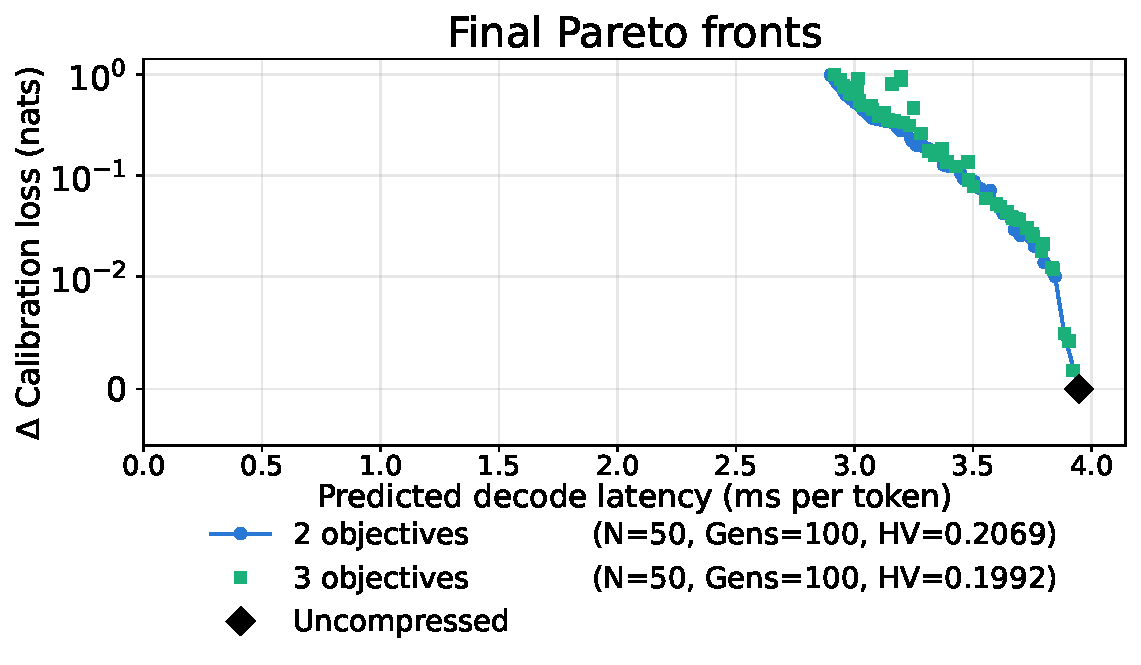
\includegraphics[width=\linewidth]{figures/a100_fronts_latency.pdf}
  \caption{Latency.}
\end{subfigure}\hfill
\begin{subfigure}{0.49\linewidth}
  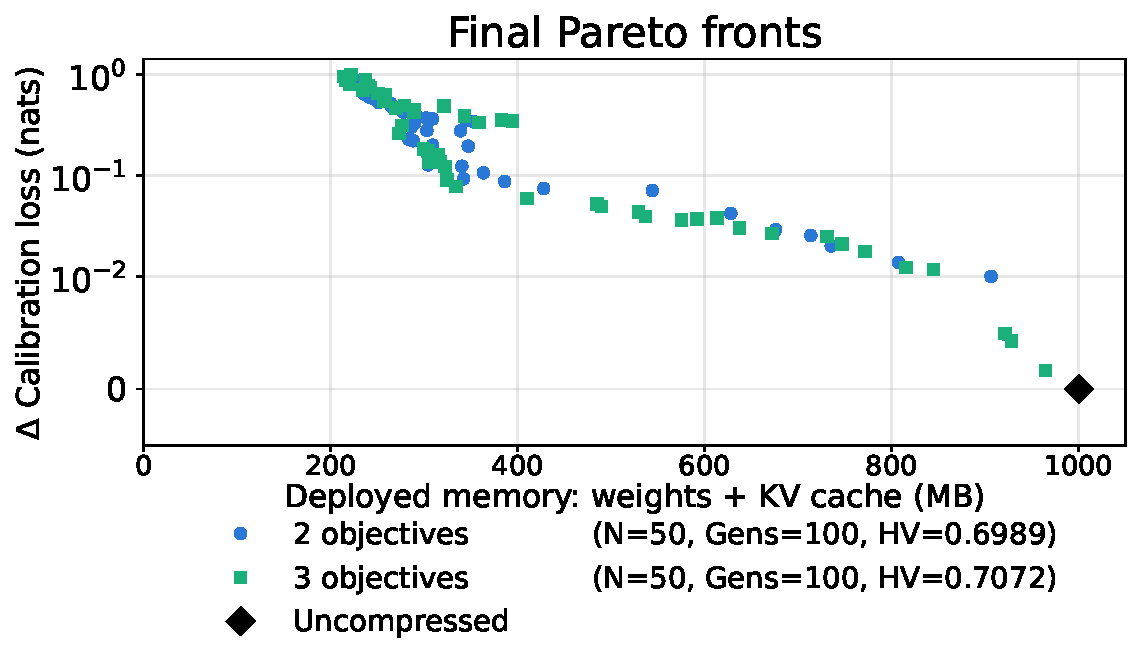
\includegraphics[width=\linewidth]{figures/a100_fronts_memory.pdf}
  \caption{Memory.}
\end{subfigure}\\[6pt]
\begin{subfigure}{0.72\linewidth}
  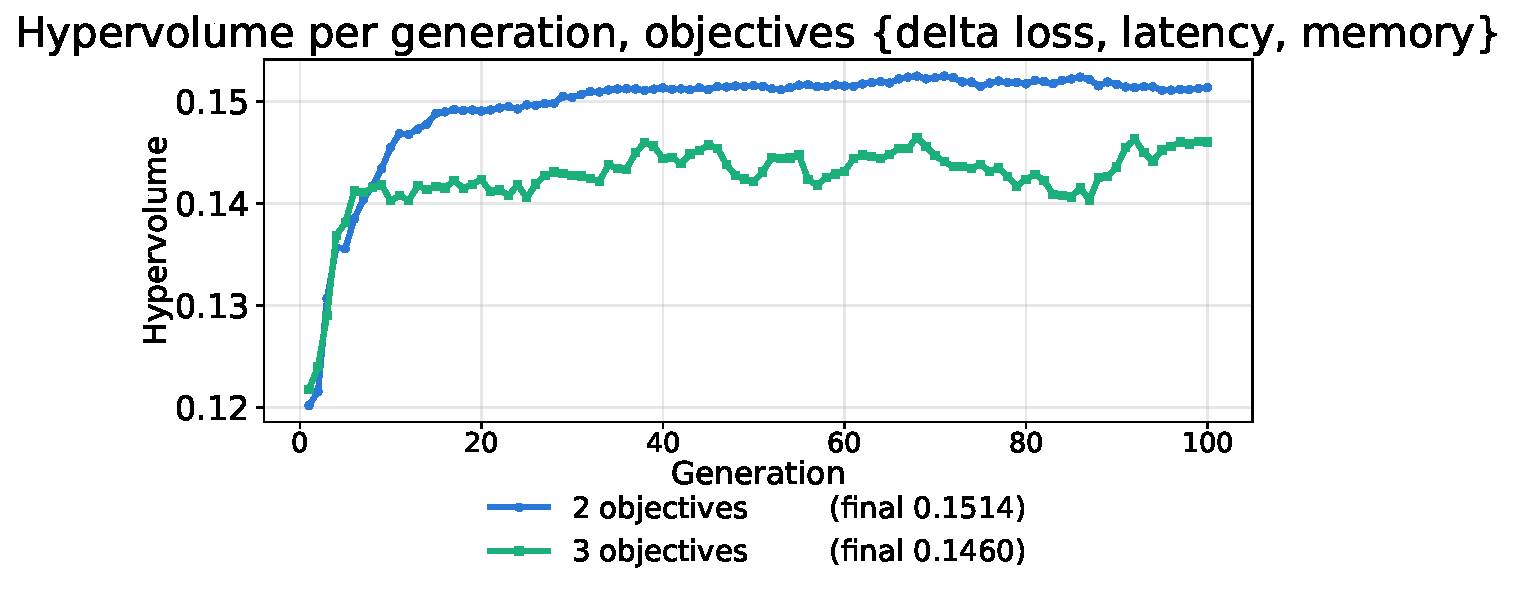
\includegraphics[width=\linewidth]{figures/a100_hv_3d.pdf}
  \caption{Hypervolume in \{loss, latency, memory\}.}
\end{subfigure}
\end{adjustbox}
\caption{Final fronts of the two A100 searches against predicted decode latency (a) and deployed memory
(b), and their hypervolume per generation with one shared normalization (c).}\label{fig:a100-compare}
\end{figure}
\end{frame}

\begin{frame}{Mixing sharing, pruning and formats}{The turn time barely changes}
\begin{table}
\centering
\begin{adjustbox}{width=\linewidth, totalheight=0.64\textheight, keepaspectratio, center}
\centering
\small
\begin{tabular}{lcccc}
\toprule
& \multicolumn{2}{c}{bf16} & \multicolumn{2}{c}{int4, group 128} \\
\cmidrule(lr){2-3}\cmidrule(lr){4-5}
GPU operation & ms & share & ms & share \\
\midrule
Attention over the KV cache, prompt tokens        & 567  & 56\% & 567  & 54\% \\
Attention over the KV cache, generated tokens     & 102  & 10\% & 102  & 10\% \\
Fixed parts, norms, activations, residuals        & 212  & 21\% & 212  & 20\% \\
Attention and MLP products, prompt tokens         & 16   & 2\%  & 91   & 9\%  \\
Attention and MLP products, generated tokens      & 107  & 10\% & 74   & 7\%  \\
Output head, generated tokens                     & 13   & 1\%  & 8    & 1\%  \\
\midrule
Total                                             & 1018 &      & 1054 &      \\
\bottomrule
\end{tabular}
\end{adjustbox}
\caption{Where the GPU time of one agent turn goes: Qwen2.5-0.5B-Instruct on the A100 reads 2000 new prompt
tokens and generates 300 tokens, over 32{,}000 tokens of context, with 4 agents decoding together
(Eq.~\ref{R-eq:turn}; predicted).}\label{tab:turn}
\end{table}
\end{frame}

\begin{frame}{Mixing sharing, pruning and formats}{Stored size against GPU memory}
\begin{table}
\centering
\begin{adjustbox}{width=\linewidth, totalheight=0.64\textheight, keepaspectratio, center}
\centering
\small
\begin{tabular}{rccc}
\toprule
$\dloss$ & Mix: smallest & Same solution, & 3 obj.: smallest \\
(nats) & stored (MB) & deployed (MB) & deployed (MB) \\
\midrule
0.02 & 374 & 966 & 725 \\
0.05 & 312 & 873 & 430 \\
0.1  & 272 & 423 & 299 \\
0.2  & 235 & 417 & 263 \\
0.5  & 187 & 793 & 228 \\
1.0  & 158 & 654 & 202 \\
\bottomrule
\end{tabular}
\end{adjustbox}
\caption{Stored size of the mixed search against deployed weights, over all evaluated solutions,
without the KV cache. The uncompressed model takes 988\,MB in both columns.}\label{tab:mix-size}
\end{table}
\end{frame}

\begin{frame}{Mixing sharing, pruning and formats}{Stored size against GPU memory}
\begin{figure}
\centering
\begin{adjustbox}{minipage=\linewidth, max width=\linewidth, max totalheight=0.76\textheight, center}
\centering
\begin{subfigure}{0.49\linewidth}
  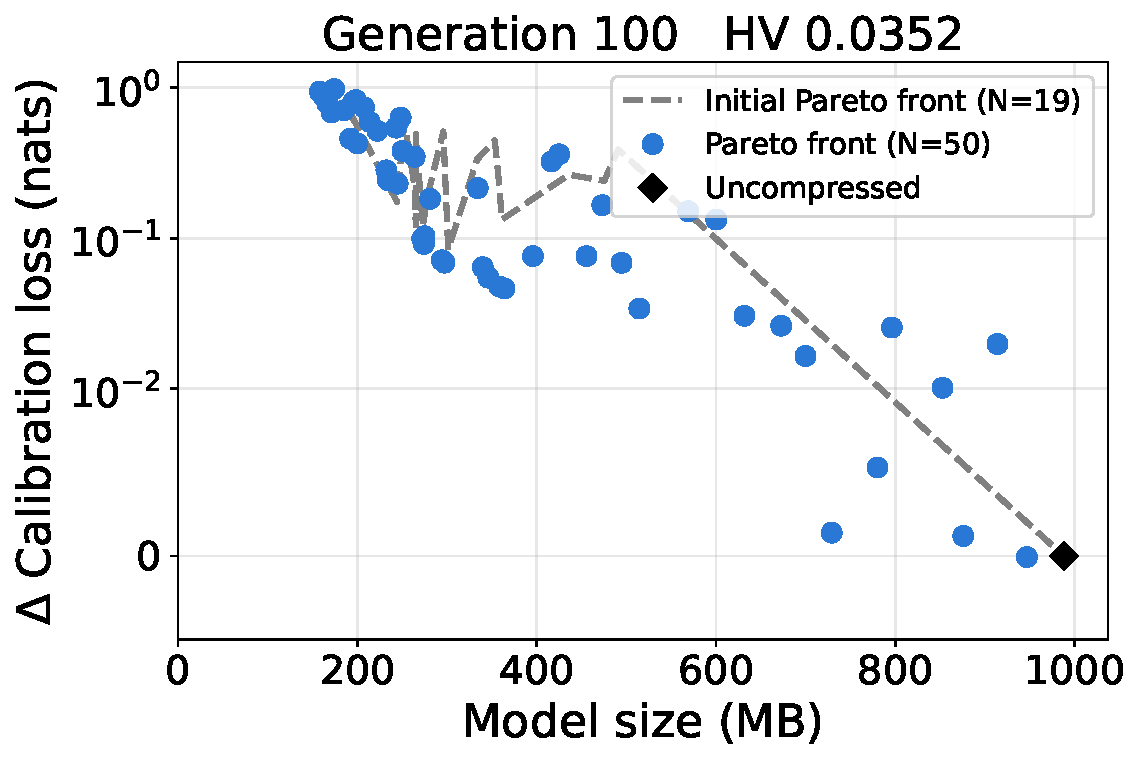
\includegraphics[width=\linewidth]{figures/mix_front_size.pdf}
  \caption{Stored size (objective).}
\end{subfigure}\hfill
\begin{subfigure}{0.49\linewidth}
  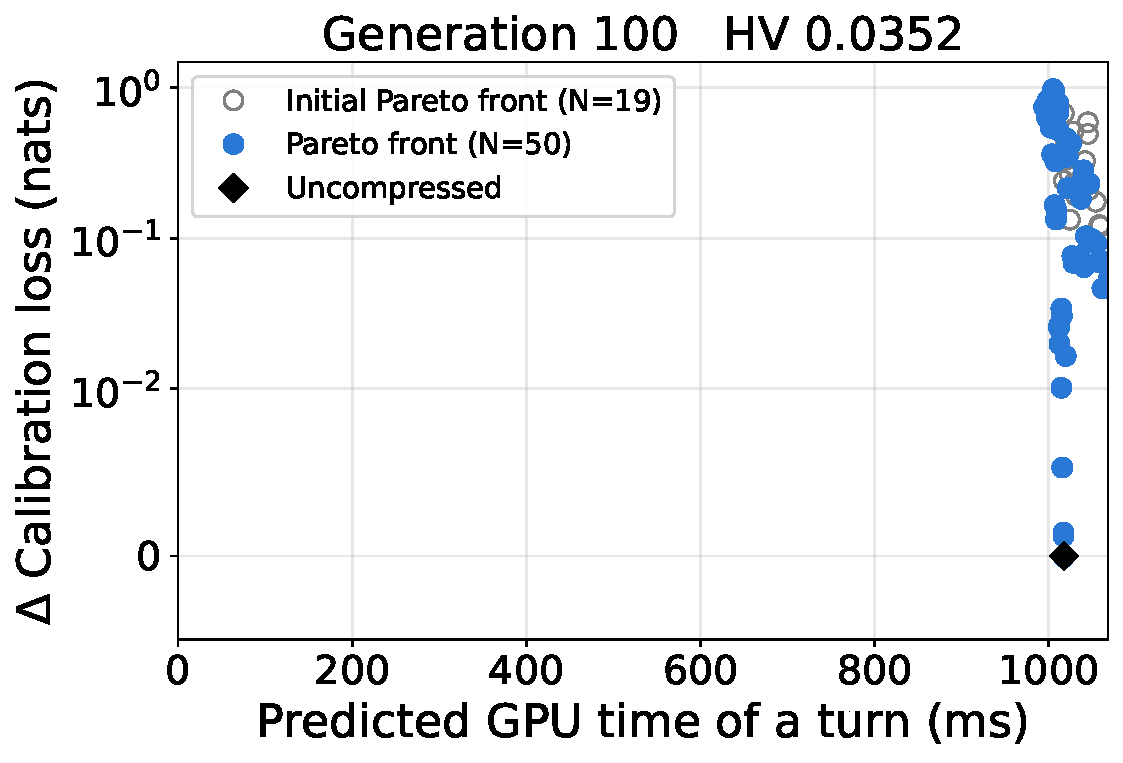
\includegraphics[width=\linewidth]{figures/mix_front_time.pdf}
  \caption{GPU time of a turn (objective).}
\end{subfigure}\\[6pt]
\begin{subfigure}{0.49\linewidth}
  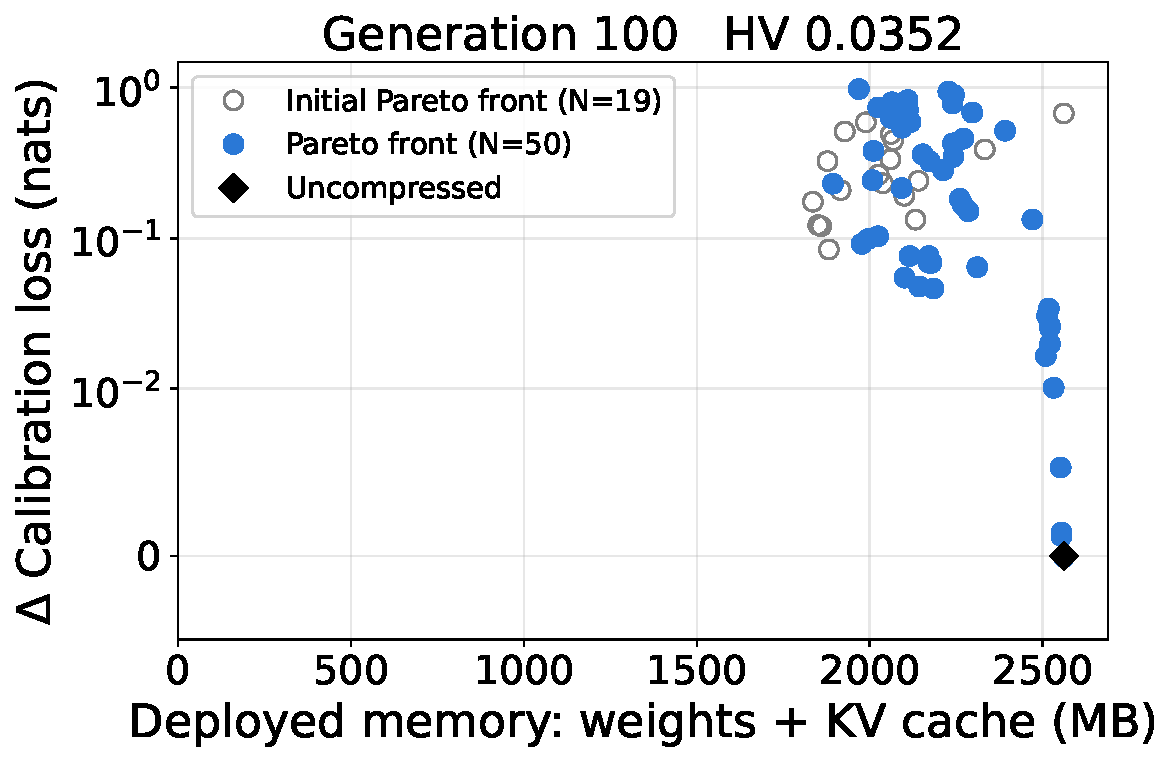
\includegraphics[width=\linewidth]{figures/mix_front_memory.pdf}
  \caption{Deployed memory, 4 agents (reported).}
\end{subfigure}\hfill
\begin{subfigure}{0.49\linewidth}
  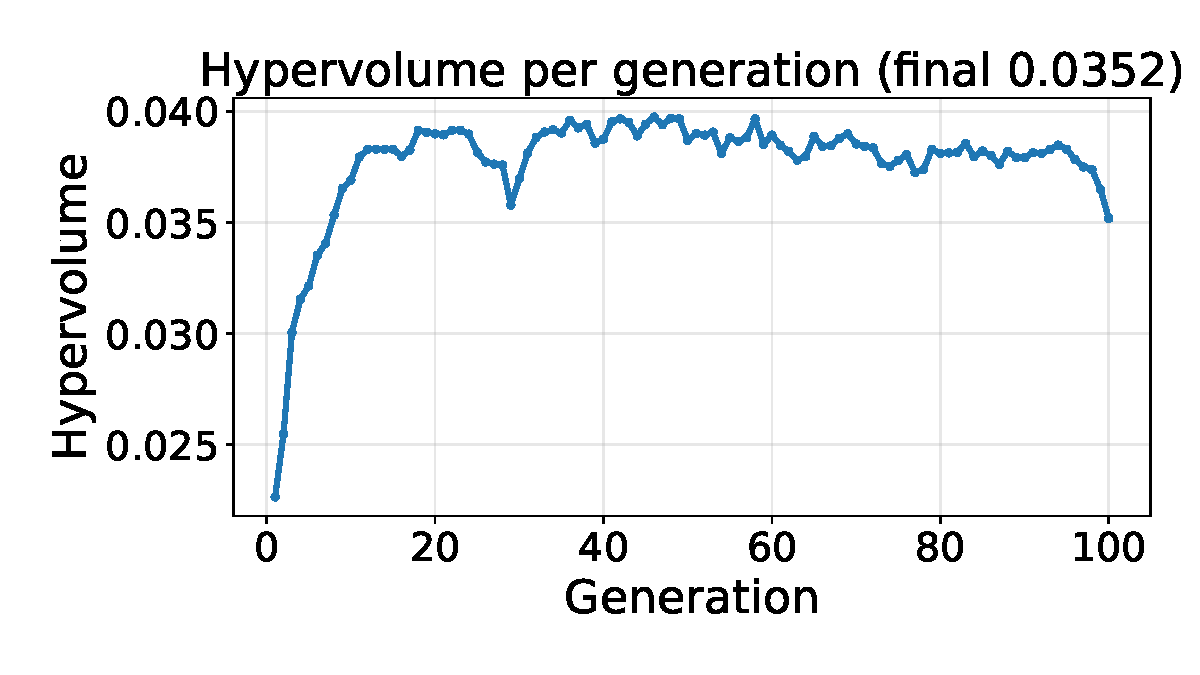
\includegraphics[width=\linewidth]{figures/mix_hv.pdf}
  \caption{Hypervolume per generation.}
\end{subfigure}
\end{adjustbox}
\caption{Mixed search: final front (50 solutions), initial front and the uncompressed model. A front in
three objectives is not ordered along any one axis, so it does not form a curve in these projections.}\label{fig:mix-front}
\end{figure}
\end{frame}

\begin{frame}{Mixing sharing, pruning and formats}{Test perplexity}
\begin{table}
\centering
\begin{adjustbox}{width=\linewidth, totalheight=0.64\textheight, keepaspectratio, center}
\centering
\small
\begin{tabular}{rccccc}
\toprule
Turn (ms) & Stored (MB) & Deployed, 4 agents (MB) & $\dloss$ (nats) & WikiText-2 & C4 \\
\midrule
 1018 (1.00$\times$) & 988 & 2561 & 0     & 14.34 & 22.33 \\
\midrule
 1013 (1.00$\times$) & 914 & 2521 & 0.020 & 14.82 & 22.81 \\
 1070 (0.95$\times$) & 346 & 2101 & 0.055 & 15.56 & 23.84 \\
 1040 (0.98$\times$) & 232 & 2212 & 0.283 & 20.04 & 31.21 \\
 1021 (1.00$\times$) & 192 & 2270 & 0.459 & 27.55 & 39.67 \\
 1007 (1.01$\times$) & 214 & 2117 & 0.592 & 35.71 & 48.86 \\
 995 (1.02$\times$) & 207 & 2024 & 0.740 & 49.49 & 65.61 \\
\bottomrule
\end{tabular}
\end{adjustbox}
\caption{Test perplexity (32 windows of 2048 tokens each) of the uncompressed model and of points of the
final front of the mixed search. In parentheses: the speedup over the uncompressed model (1018\,ms).}\label{tab:mix-test}
\end{table}
\end{frame}

\begin{frame}{Mixing sharing, pruning and formats}{Test perplexity}
\begin{figure}
\centering
\begin{adjustbox}{minipage=\linewidth, max width=\linewidth, max totalheight=0.76\textheight, center}
\centering
\begin{subfigure}{0.49\linewidth}
  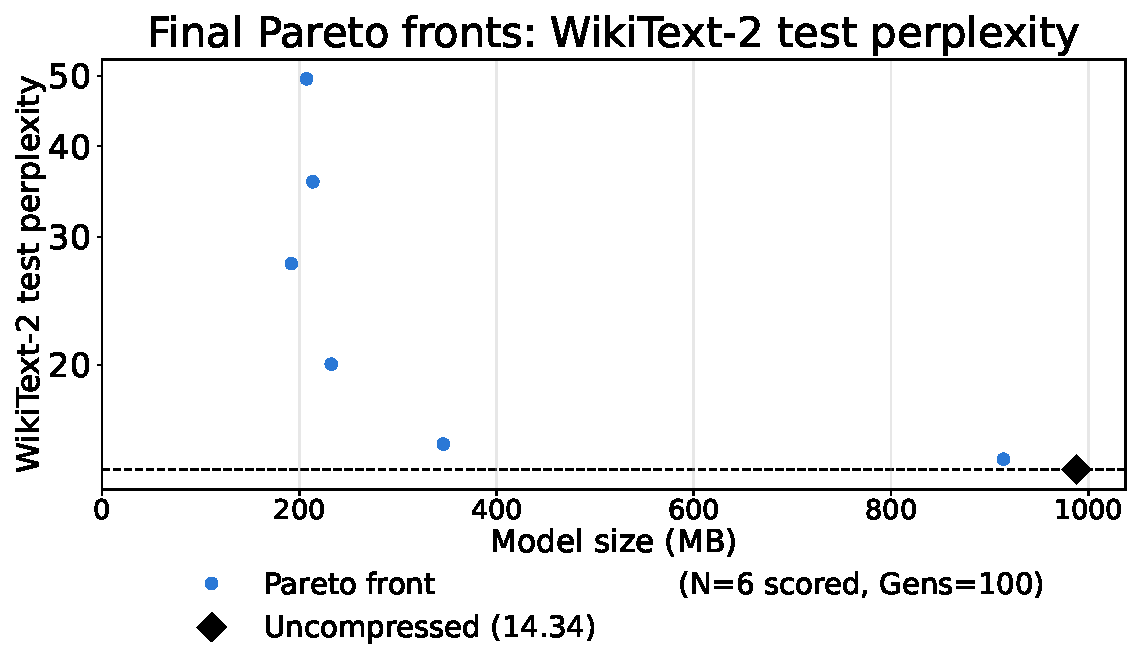
\includegraphics[width=\linewidth]{figures/mix_test_wikitext2.pdf}
  \caption{WikiText-2 test.}
\end{subfigure}\hfill
\begin{subfigure}{0.49\linewidth}
  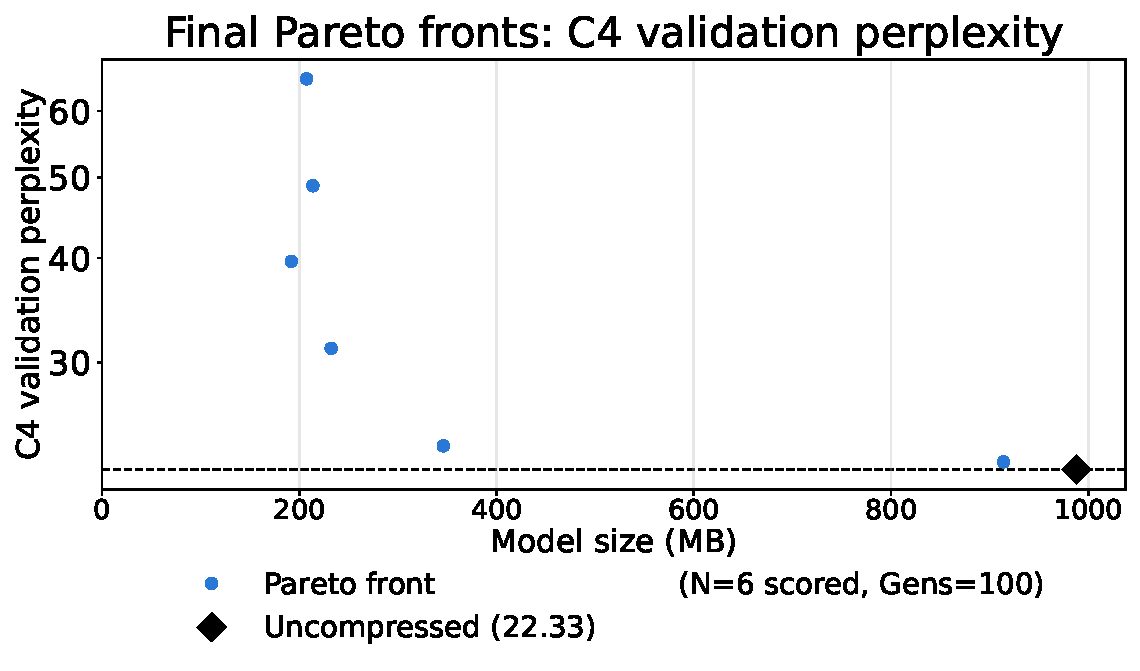
\includegraphics[width=\linewidth]{figures/mix_test_c4.pdf}
  \caption{C4 validation.}
\end{subfigure}
\end{adjustbox}
\caption{Test perplexity of the scored points of the mixed search against stored size.}\label{fig:mix-test}
\end{figure}
\end{frame}

\begin{frame}{The KV cache as a decision}{Probing the cache formats}
\begin{table}
\centering
\begin{adjustbox}{width=\linewidth, totalheight=0.64\textheight, keepaspectratio, center}
\centering
\small
\begin{tabular}{lcc}
\toprule
Cache setting (all layers) & $\dloss$ (nats) & Facts recalled \\
\midrule
Uncompressed                                         & 0       & 100\% \\
\midrule
Keys int8, one scale per token                       & +0.037  & 100\% \\
Keys int8, one scale per channel (int8c)             & +0.0004 & 100\% \\
Keys int4, one scale per token                       & +1.614  & 6\%   \\
Keys int4, one scale per channel (int4c)             & +0.070  & 100\% \\
Values int8 / int4 (per token)                       & $-$0.001 / +0.008 & 100\% \\
Keys or values int2 (any scaling)                    & +1.18 to +6.01 & 0\% \\
Keys int4c, values int4                              & +0.077  & 98\%  \\
\midrule
Window 0.75, plain                                   & +0.868  & 22\%  \\
Window 0.75, first token kept                        & +0.004  & 69\%  \\
Window 0.5, first token kept                         & +0.010  & 52\%  \\
Window 0.25, first token kept                        & +0.039  & 14\%  \\
Window 0.125, first token kept                       & +0.084  & 2\%   \\
Window 0.25, band 0 or band 3 at full context        & +0.037 / +0.026 & 14\% \\
Window 0.125, every 4th layer at full context        & +0.080  & 2\%   \\
\bottomrule
\end{tabular}
\end{adjustbox}
\caption{KV probe on the A100: calibration loss increase and planted facts recalled (64 facts, so about
$\pm6$ points), with one setting for all layers unless stated.}\label{tab:kv-probe}
\end{table}
\end{frame}

\begin{frame}{The KV cache as a decision}{Second search: per-channel keys, recall as a constraint}
\begin{table}
\centering
\begin{adjustbox}{width=\linewidth, totalheight=0.64\textheight, keepaspectratio, center}
\centering
\small
\begin{tabular}{rccccc}
\toprule
& \multicolumn{2}{c}{First search (no recall check)} & \multicolumn{3}{c}{Second search (recall $\ge95\%$)} \\
\cmidrule(lr){2-3}\cmidrule(lr){4-6}
$\dloss$ (nats) & Fastest (ms) & Smallest (MB) & Fastest (ms) & Smallest (MB) & Agents \\
\midrule
0 (uncompressed) & 1021 (1.00$\times$) & 2561 & 1019 (1.00$\times$) & 2561 & 180 \\
\midrule
0.01 & 1019 (1.00$\times$) & 2049 & 868 (1.17$\times$) & 1566 & 491 \\
0.02 & 971 (1.05$\times$) & 2035 & 821 (1.24$\times$) & 1443 & 520 \\
0.05 & 933 (1.09$\times$) & 1591 & 819 (1.24$\times$) & 1152 & 789 \\
0.1  & 883 (1.16$\times$) & 1147 & 807 (1.26$\times$) &  815 & 854 \\
0.2  & 808 (1.26$\times$) &  914 & 807 (1.26$\times$) &  705 & 772 \\
\bottomrule
\end{tabular}
\end{adjustbox}
\caption{The KV searches: predicted GPU time of a turn of the fastest solution and deployed memory (weights
and the cache of 4 agents) of the smallest one within each calibration-loss budget, over all evaluations.
Agents: how many fit on 80\,GB with the smallest solution of the second search. In parentheses: the speedup over the uncompressed model as each search timed it (1021 and 1019\,ms).}\label{tab:kv-limits}
\end{table}
\end{frame}

\begin{frame}{The KV cache as a decision}{Second search: per-channel keys, recall as a constraint}
\begin{figure}
\centering
\begin{adjustbox}{minipage=\linewidth, max width=\linewidth, max totalheight=0.76\textheight, center}
\centering
\begin{subfigure}{0.49\linewidth}
  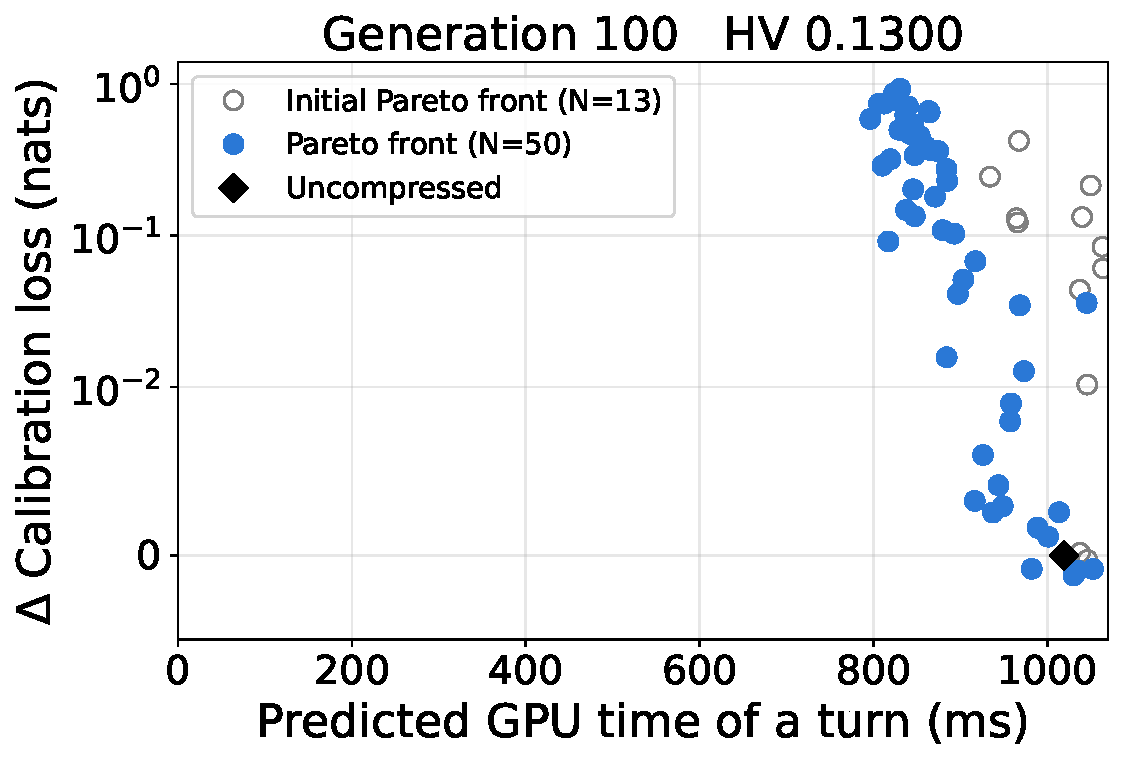
\includegraphics[width=\linewidth]{figures/kv2_front_time.pdf}
  \caption{GPU time of a turn (objective).}
\end{subfigure}\hfill
\begin{subfigure}{0.49\linewidth}
  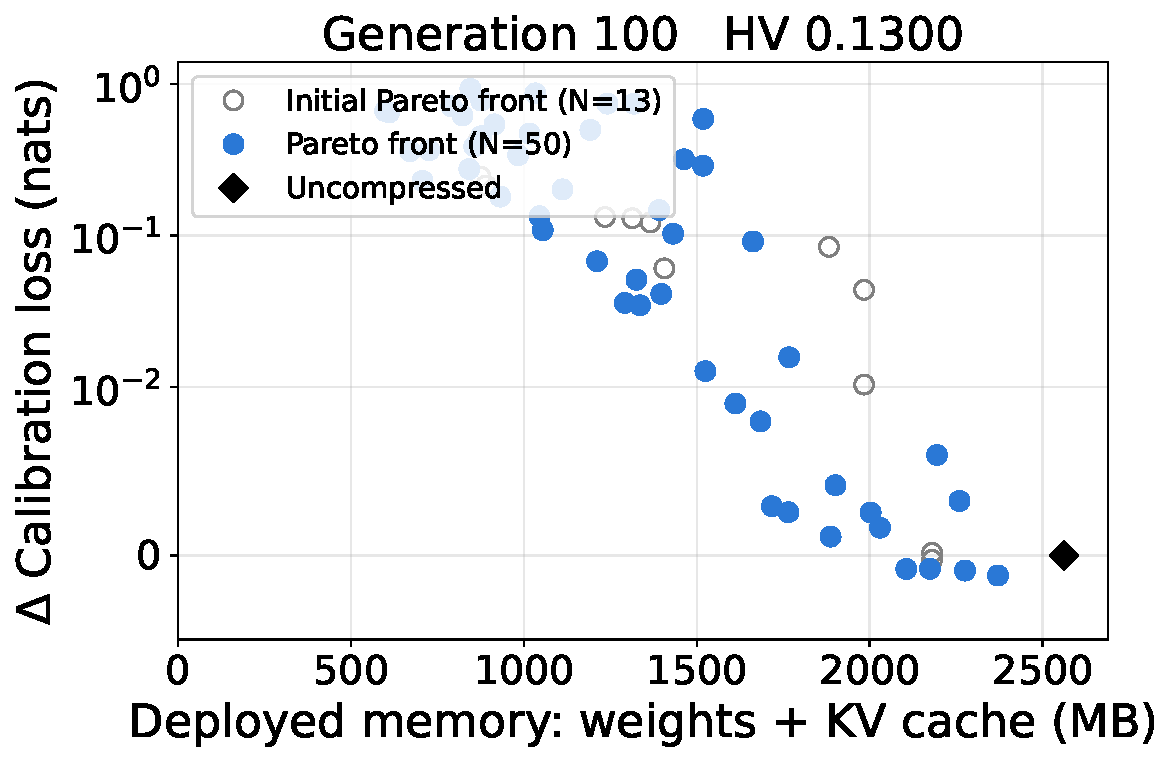
\includegraphics[width=\linewidth]{figures/kv2_front_memory.pdf}
  \caption{Deployed memory, 4 agents (objective).}
\end{subfigure}\\[6pt]
\begin{subfigure}{0.49\linewidth}
  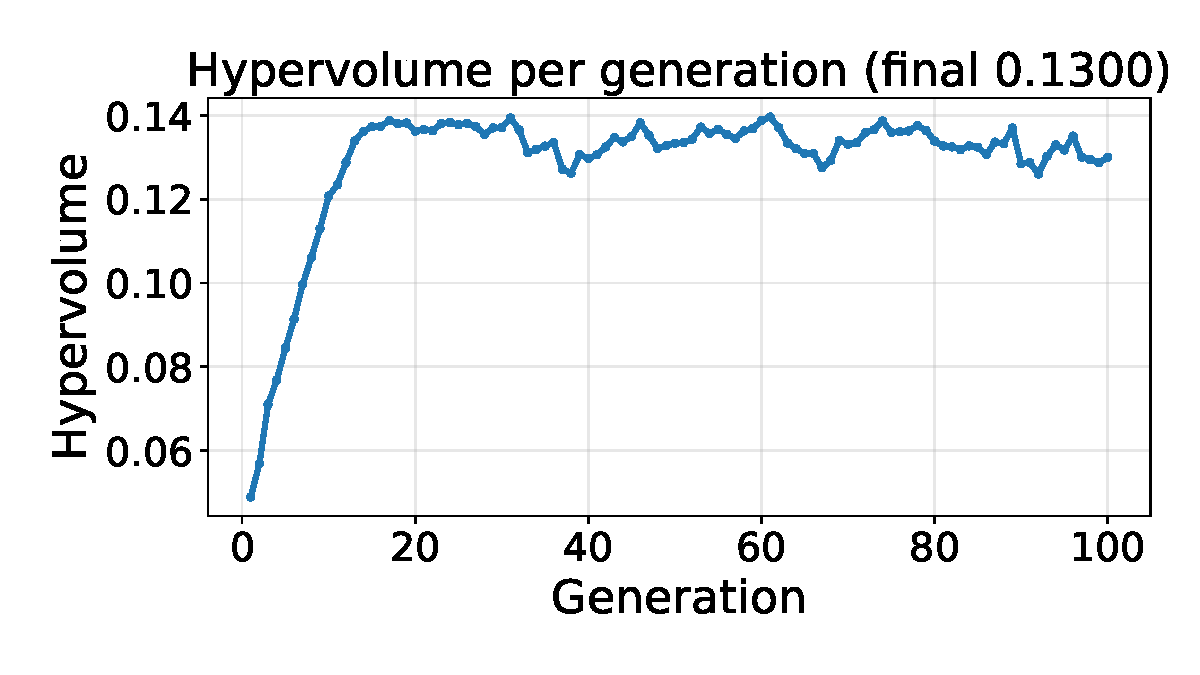
\includegraphics[width=\linewidth]{figures/kv2_hv.pdf}
  \caption{Hypervolume per generation.}
\end{subfigure}\hfill
\begin{subfigure}{0.49\linewidth}
  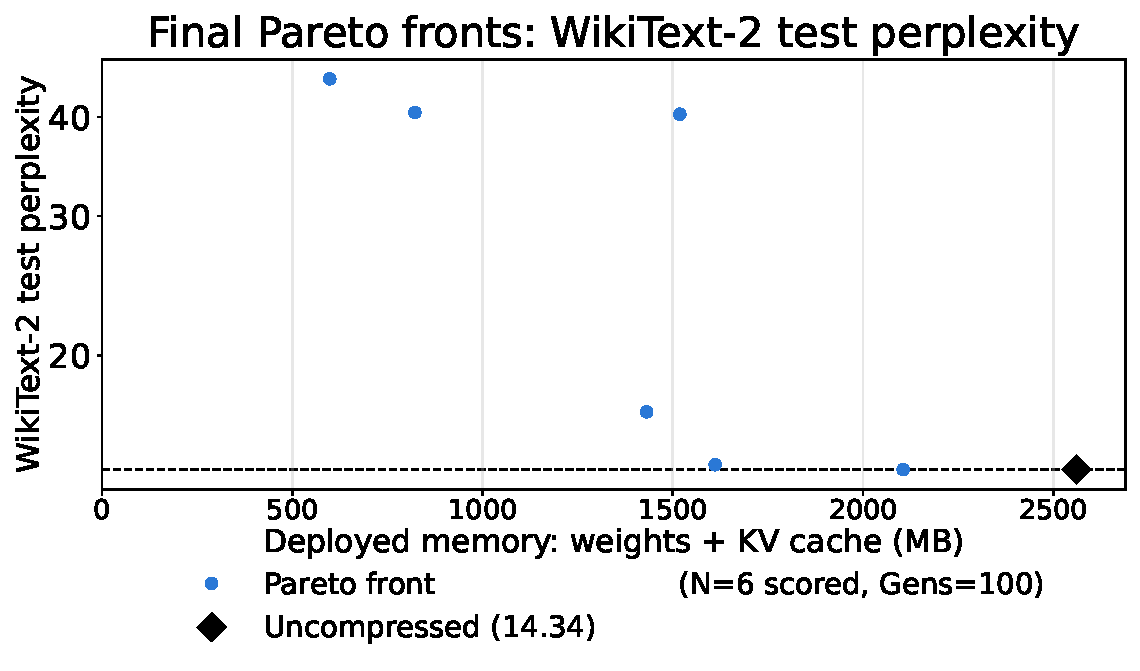
\includegraphics[width=\linewidth]{figures/kv2_test_wikitext2.pdf}
  \caption{WikiText-2 test perplexity of scored points.}
\end{subfigure}
\end{adjustbox}
\caption{Second KV search: final front (50 solutions), initial front and the uncompressed model.}\label{fig:kv2-front}
\end{figure}
\end{frame}

\begin{frame}{The KV cache as a decision}{Second search: per-channel keys, recall as a constraint}
\begin{table}
\centering
\begin{adjustbox}{width=\linewidth, totalheight=0.64\textheight, keepaspectratio, center}
\centering
\small
\begin{tabular}{rccccc}
\toprule
Turn (ms) & Deployed, 4 agents (MB) & $\dloss$ (nats) & Recall & WikiText-2 & C4 \\
\midrule
 1019 (1.00$\times$) & 2561 & 0       & 100\% & 14.34 & 22.33 \\
\midrule
 1053 (0.97$\times$) & 2106 & $-$0.001 & 100\% & 14.34 & 22.33 \\
 958 (1.06$\times$) & 1611 & 0.009   & 100\% & 14.55 & 22.54 \\
 893 (1.14$\times$) & 1431 & 0.103   & 100\% & 16.97 & 25.19 \\
 864 (1.18$\times$) &  599 & 0.664   & 98\%  & 44.72 & 51.45 \\
 837 (1.22$\times$) &  822 & 0.622   & 98\%  & 40.55 & 49.55 \\
 796 (1.28$\times$) & 1519 & 0.588   & 100\% & 40.35 & 48.08 \\
\bottomrule
\end{tabular}
\end{adjustbox}
\caption{Test perplexity (32 windows of 2048 tokens each) of the uncompressed model and of the scored points
of the second KV search's final front; recall on the search's 64 facts. In parentheses: the speedup over the uncompressed model (1019\,ms).}\label{tab:kv2-test}
\end{table}
\end{frame}

\begin{frame}{The KV cache as a decision}{Re-check: a second kernel, aligned windows and new facts}
\begin{table}
\centering
\begin{adjustbox}{width=\linewidth, totalheight=0.64\textheight, keepaspectratio, center}
\centering
\small
\begin{tabular}{lcccc}
\toprule
& \multicolumn{2}{c}{32{,}000 tokens} & \multicolumn{2}{c}{Window 0.25 (8001 / 8064 tokens)} \\
\cmidrule(lr){2-3}\cmidrule(lr){4-5}
Cache: keys / values & First kernel & Second kernel & First kernel & Second kernel \\
\midrule
bf16 / bf16, PyTorch attention & 59.7 & 57.9 & 25.7 & 26.0 \\
bf16 / bf16                    & 69.4 & 48.5 & 38.0 & 16.4 \\
bf16 / int8                    & 69.3 & 42.9 & 39.5 & 16.3 \\
bf16 / int4                    & 65.5 & 38.6 & 37.9 & 15.9 \\
int8c / bf16                   & 62.2 & 61.6 & 37.3 & 22.1 \\
int8c / int8                   & 66.5 & 59.2 & 38.8 & 23.0 \\
int8c / int4                   & 64.2 & 55.6 & 38.3 & 22.3 \\
int4c / bf16                   & 58.8 & 55.9 & 36.6 & 20.6 \\
int4c / int8                   & 65.2 & 53.9 & 38.2 & 21.5 \\
int4c / int4                   & 64.4 & 50.7 & 37.8 & 21.5 \\
\bottomrule
\end{tabular}
\end{adjustbox}
\caption{Decode attention per layer and step (\us) on the A100, 4 sequences, with the cache read in place by
the two Triton kernels. The windows were timed at 8001 tokens by the search and at an aligned 8064 by the
re-check.}\label{tab:kv-kernel}
\end{table}
\end{frame}

\begin{frame}{The KV cache as a decision}{Re-check: a second kernel, aligned windows and new facts}
\begin{table}
\centering
\begin{adjustbox}{width=\linewidth, totalheight=0.64\textheight, keepaspectratio, center}
\centering
\small
\begin{tabular}{rcccc}
\toprule
& \multicolumn{2}{c}{Fastest} & \multicolumn{2}{c}{Smallest} \\
\cmidrule(lr){2-3}\cmidrule(lr){4-5}
$\dloss$ (nats) & As searched (ms) & Re-timed (ms) & Memory (MB) & Agents \\
\midrule
0 (uncompressed) & 1019 (1.00$\times$) & 1000 (1.00$\times$) & 2561 & 180 \\
\midrule
0.01 & 868 (1.17$\times$) & 793 (1.26$\times$) & 1566 & 491 \\
0.02 & 821 (1.24$\times$) & 757 (1.32$\times$) & 1443 & 520 \\
0.05 & 819 (1.24$\times$) & 752 (1.33$\times$) & 1152 & 789 \\
0.1  & 807 (1.26$\times$) & 749 (1.33$\times$) &  815 & 854 \\
0.2  & 807 (1.26$\times$) & 747 (1.34$\times$) &  705 & 772 \\
\bottomrule
\end{tabular}
\end{adjustbox}
\caption{Second KV search re-timed with the second kernel and aligned windows: the predicted GPU time of a
turn of the fastest feasible solution within each budget (the fastest may be another solution after
re-timing), and the deployed memory of the smallest one (4 agents) with the agents that fit on 80\,GB.
In parentheses: the speedup over the uncompressed model as the search and the re-check timed it (1019 and
1000\,ms).}\label{tab:kv-retimed}
\end{table}
\end{frame}

\begin{frame}{The KV cache as a decision}{Re-check: a second kernel, aligned windows and new facts}
\begin{table}
\centering
\begin{adjustbox}{width=\linewidth, totalheight=0.64\textheight, keepaspectratio, center}
\centering
\footnotesize
\setlength{\tabcolsep}{4pt}
\begin{tabular}{lcccccc}
\toprule
& & & & \multicolumn{2}{c}{Recall} & \\
\cmidrule(lr){5-6}
Configuration & $\dloss$ (nats) & Turn (ms) & Memory (MB) & Search's 64 & New 256 & Windows \\
\midrule
uncompressed                 & 0      & 1000 (1.00$\times$) & 2561 & 100\% & 100.0\% & 1/1/1/1 \\
\midrule
fastest within 0.01 nats     & 0.0064 & 793 (1.26$\times$) & 2063 & 100\% & 100.0\% & 0.25/1/1/0.5 \\
fastest within 0.02 nats     & 0.0174 & 757 (1.32$\times$) & 1941 & 100\% & 100.0\% & 0.25/1/1/0.25 \\
fastest within 0.05 nats     & 0.0371 & 752 (1.33$\times$) & 1471 & 100\% & 100.0\% & 0.25/1/1/0.25 \\
fastest within 0.1 nats      & 0.0556 & 749 (1.33$\times$) & 1746 & 100\% & 100.0\% & 0.25/1/1/0.25 \\
fastest within 0.2 nats      & 0.1522 & 747 (1.34$\times$) & 1381 & 100\% & 100.0\% & 0.25/1/1/0.25 \\
\midrule
smallest within 0.01 nats    & 0.0071 & 812 (1.23$\times$) & 1566 & 100\% & 100.0\% & 0.25/1/1/0.5 \\
smallest within 0.02 nats    & 0.0198 & 908 (1.10$\times$) & 1443 & 100\% & 99.6\%  & 0.5/1/1/0.75 \\
smallest within 0.05 nats    & 0.0484 & 847 (1.18$\times$) & 1152 & 100\% & 99.2\%  & 0.25/1/1/0.5 \\
smallest within 0.1 nats     & 0.0997 & 817 (1.22$\times$) &  815 & 98\%  & 99.6\%  & 0.25/1/1/0.25 \\
smallest within 0.2 nats     & 0.1728 & 822 (1.22$\times$) &  705 & 97\%  & 98.4\%  & 0.25/1/1/0.25 \\
\bottomrule
\end{tabular}
\end{adjustbox}
\caption{Recall of planted facts by the solutions of Table~\ref{tab:kv-retimed}: on the 64 facts in
calibration text the search selected on, and on 256 new facts in C4 validation text. Turn times re-timed;
windows per depth band (layers 0--5, 6--11, 12--17, 18--23). In parentheses: the speedup over the uncompressed model (1000\,ms).}\label{tab:kv-recall}
\end{table}
\end{frame}

\begin{frame}{Benchmarks: Selected UBQ-ECSQ models}{}
\begin{table}
\centering
\begin{adjustbox}{width=\linewidth, totalheight=0.64\textheight, keepaspectratio, center}
\centering
\footnotesize
\setlength{\tabcolsep}{3.5pt}
\begin{tabular}{lccccccccc}
\toprule
Model & $k$ & $c$ & Sparsity & Calib loss & Size & Bits/w & Huffman & WikiText-2 & C4 \\
($\dloss$ (\%)) &     &     & (\%)     & (\%)        & (MB) &        & bits/w  & ppl        & ppl \\
\midrule
Uncompressed (bf16) & --  & --    & 0.0  & 0.00 & 988 (1.00$\times$) & 16.00 & --   & 14.26 & 21.46 \\
\addlinespace
Q0  (0\%)  & 164 & 0.995 & 2.2  & 0.12 & 495 (2.00$\times$) & 8.02 & 6.47 & 14.26 & 21.55 \\
Q1  (1\%)  & 65  & 0.934 & 5.3  & 1.00 & 414 (2.39$\times$) & 6.70 & 5.23 & 14.61 & 22.08 \\
Q2  (2\%)  & 52  & 0.949 & 6.8  & 1.61 & 372 (2.66$\times$) & 6.01 & 4.84 & 15.08 & 22.49 \\
Q5  (5\%)  & 29  & 0.928 & 11.8 & 4.75 & 310 (3.19$\times$) & 5.01 & 4.05 & 17.00 & 25.05 \\
Q10 (10\%) & 28  & 0.849 & 19.2 & 9.87 & 309 (3.20$\times$) & 5.00 & 3.98 & 20.52 & 29.70 \\
\bottomrule
\end{tabular}
\end{adjustbox}
\caption{Selected solutions. Sparsity counts pruned weights and weights rounded to zero. Huffman bits/w
is the storage with Huffman-coded codes (reported only, not optimized). None of the five merges levels
($\rho=1$). In parentheses after the size: the compression ratio, the uncompressed size over the model's.}\label{tab:models}
\end{table}
\end{frame}

\begin{frame}{Benchmarks: Benchmark protocol}{}
\begin{table}
\centering
\begin{adjustbox}{width=\linewidth, totalheight=0.64\textheight, keepaspectratio, center}
\centering
\footnotesize
\setlength{\tabcolsep}{4pt}
\begin{tabular}{l>{\raggedright\arraybackslash}p{7.2cm}cccc}
\toprule
Benchmark & What it tests & Split & Questions & Shots & Metric \\
\midrule
PIQA          & Physical commonsense: the right way to do an everyday task & validation & 1{,}838 & 0 & acc.\ (norm.) \\
ARC-Easy      & Grade-school science questions & test & 2{,}376 & 0 & acc.\ (norm.) \\
ARC-Challenge & Harder grade-school science questions (retrieval-resistant) & test & 1{,}172 & 0 & acc.\ (norm.) \\
HellaSwag     & Commonsense: the most plausible continuation of an everyday scene & validation & 10{,}042 & 0 & acc.\ (norm.) \\
WinoGrande    & Commonsense pronoun resolution (fill in the blank, two options) & validation & 1{,}267 & 0 & accuracy \\
BoolQ         & Reading comprehension: yes/no questions about a Wikipedia passage & validation & 3{,}270 & 0 & accuracy \\
MMLU          & Knowledge and reasoning in 57 subjects (STEM, humanities, law, medicine, \dots) & test & 14{,}042 & 5 & accuracy \\
GSM8K         & Multi-step grade-school math word problems, solved in writing & test & 1{,}319 & 5 & exact match \\
\bottomrule
\end{tabular}
\end{adjustbox}
\caption{Benchmarks. Multiple-choice tasks pick the answer with the highest log-likelihood (acc.\ (norm.):
log-likelihood normalized by answer length); GSM8K generates a solution and compares the extracted final
number with the reference.}\label{tab:protocol}
\end{table}
\end{frame}

\begin{frame}{Benchmarks: UBQ-ECSQ results}{}
\begin{table}
\centering
\begin{adjustbox}{width=\linewidth, totalheight=0.64\textheight, keepaspectratio, center}
\centering
\small
\setlength{\tabcolsep}{4pt}
\begin{tabular}{lcccccccccc}
\toprule
Model & Size & PIQA & ARC-e & ARC-c & HellaS. & WinoG. & BoolQ & MMLU & GSM8K & Average \\
($\dloss$ (\%)) & (MB) &      &       &       &         &        &       & 5-shot & 5-shot &       \\
\midrule
Uncompressed & 988 & 70.4 & 59.2 & 33.1 & 52.4 & 56.0 & 67.8 & 47.0 & 31.2 & 52.1 \\
\addlinespace
Q0  (0\%)    & 495 & 70.2 & 59.9 & 33.5 & 52.4 & 56.6 & 68.4 & 47.0 & 31.7 & 52.5 \\
Q1  (1\%)    & 414 & 70.2 & 59.6 & 33.7 & 52.5 & 55.9 & 64.3 & 46.5 & 27.6 & 51.3 \\
Q2  (2\%)    & 372 & 69.5 & 61.0 & 32.8 & 52.0 & 54.2 & 66.6 & 46.1 & 26.7 & 51.1 \\
Q5  (5\%)    & 310 & 69.2 & 55.2 & 32.0 & 50.0 & 56.4 & 49.7 & 45.0 &  9.7 & 45.9 \\
Q10 (10\%)   & 309 & 67.5 & 56.2 & 31.0 & 47.7 & 57.2 & 56.1 & 38.3 & 12.6 & 45.8 \\
\midrule
Std. error   &     & 1.1  & 1.0  & 1.4  & 0.5  & 1.4  & 0.8  & 0.4  & 1.3  &      \\
\bottomrule
\end{tabular}
\end{adjustbox}
\caption{Accuracy (\%, higher is better), with the unweighted average over the eight benchmarks. Last
row: standard error of the uncompressed model's accuracy.}\label{tab:results}
\end{table}
\end{frame}

\begin{frame}{Benchmarks: UBQ-ECSQ results}{}
\begin{table}
\centering
\begin{adjustbox}{width=\linewidth, totalheight=0.64\textheight, keepaspectratio, center}
\centering
\small
\setlength{\tabcolsep}{4pt}
\begin{tabular}{lcccccccccc}
\toprule
Model & Size & PIQA & ARC-e & ARC-c & HellaS. & WinoG. & BoolQ & MMLU & GSM8K & Accuracy \\
($\dloss$ (\%)) & (MB) &      &       &       &         &        &       &      &       & retained (\%)       \\
\midrule
Q0  (0\%)  & 495 & $-0.2$ & $+0.7$ & $+0.4$ & $-0.1$ & $+0.6$ & $+0.6$  & $\phantom{+}0.0$ & $+0.5$ & 100.6 \\
Q1  (1\%)  & 414 & $-0.2$ & $+0.5$ & $+0.6$ & $\phantom{+}0.0$ & $-0.2$ & $-3.5$ & $-0.4$ & $-3.6$ & 98.4 \\
Q2  (2\%)  & 372 & $-0.9$ & $+1.9$ & $-0.3$ & $-0.5$ & $-1.8$ & $-1.2$  & $-0.8$ & $-4.5$  & 98.0 \\
Q5  (5\%)  & 310 & $-1.2$ & $-4.0$ & $-1.1$ & $-2.4$ & $+0.3$ & $-18.1$ & $-2.0$ & $-21.5$ & 88.0 \\
Q10 (10\%) & 309 & $-2.9$ & $-2.9$ & $-2.1$ & $-4.7$ & $+1.2$ & $-11.8$ & $-8.6$ & $-18.6$ & 87.9 \\
\bottomrule
\end{tabular}
\end{adjustbox}
\caption{Change in accuracy against the uncompressed model (percentage points; negative is a loss). Accuracy retained: the compressed model's average accuracy as a percentage of the uncompressed model's.}\label{tab:delta}
\end{table}
\end{frame}

\begin{frame}{Benchmarks: hardware-aware, RTX 3060}{Selected models}
\begin{table}
\centering
\begin{adjustbox}{width=\linewidth, totalheight=0.64\textheight, keepaspectratio, center}
\centering
\footnotesize
\setlength{\tabcolsep}{3.5pt}
\begin{tabular}{lcccccc}
\toprule
Model & Calib & Latency & Memory & Bits/w & int4 & Removed \\
($\dloss$ (\%)) & loss (\%) & (ms) & (MB) & & (\%) & attn./MLP \\
\midrule
Uncompressed & 0.00 & 6.78 (1.00$\times$) & 1001 (1.00$\times$) & 16.00 & 0  & 0/0 \\
\addlinespace
H0  (0\%)  & 0.16 & 6.74 (1.01$\times$) & 992 (1.01$\times$) & 15.86 & 1  & 0/0 \\
H1  (1\%)  & 0.75 & 5.61 (1.21$\times$) & 761 (1.31$\times$) & 12.13 & 35 & 0/0 \\
H2  (2\%)  & 1.99 & 4.35 (1.56$\times$) & 479 (2.09$\times$) & 7.55  & 77 & 0/0 \\
H5  (5\%)  & 4.84 & 3.43 (1.98$\times$) & 291 (3.43$\times$) & 4.51  & 99 & 0/0 \\
H10 (10\%) & 8.90 & 3.28 (2.07$\times$) & 271 (3.70$\times$) & 4.19  & 97 & 1/1 \\
\bottomrule
\end{tabular}
\end{adjustbox}
\caption{Selected hardware-aware solutions. Bits/w counts weights only; memory includes the 13\,MB KV
cache. None prunes MLP neurons. In parentheses: after the latency, the speedup over the uncompressed model
(6.78\,ms); after the memory, the compression ratio (the uncompressed model's memory over this model's).}\label{tab:hwmodels}
\end{table}
\end{frame}

\begin{frame}{Benchmarks: hardware-aware, RTX 3060}{Results}
\begin{table}
\centering
\begin{adjustbox}{width=\linewidth, totalheight=0.64\textheight, keepaspectratio, center}
\centering
\small
\setlength{\tabcolsep}{3pt}
\begin{tabular}{lcccccccccc}
\toprule
Model & Latency & PIQA & ARC-e & ARC-c & HellaS. & WinoG. & BoolQ & MMLU & GSM8K & Average \\
($\dloss$ (\%)) & (ms)   &      &       &       &         &        &       & 5-shot & 5-shot & \\
\midrule
Uncompressed & 6.78 (1.00$\times$) & 70.6 & 59.2 & 33.0 & 52.4 & 55.2 & 67.7 & 47.0 & 30.3 & 51.9 \\
\addlinespace
H0  (0\%)    & 6.74 (1.01$\times$) & 70.7 & 59.6 & 33.4 & 52.0 & 55.6 & 66.9 & 46.5 & 31.1 & 52.0 \\
H1  (1\%)    & 5.61 (1.21$\times$) & 70.1 & 60.0 & 32.7 & 51.4 & 56.0 & 67.6 & 46.7 & 27.9 & 51.5 \\
H2  (2\%)    & 4.35 (1.56$\times$) & 69.7 & 59.7 & 32.8 & 51.0 & 56.7 & 66.1 & 45.9 & 28.5 & 51.3 \\
H5  (5\%)    & 3.43 (1.98$\times$) & 69.0 & 58.0 & 31.5 & 49.4 & 55.0 & 66.5 & 44.8 & 20.5 & 49.4 \\
H10 (10\%)   & 3.28 (2.07$\times$) & 67.3 & 49.7 & 29.0 & 46.4 & 52.4 & 63.8 & 37.6 &  4.9 & 43.9 \\
\midrule
Std. error   &      & 1.1  & 1.0  & 1.4  & 0.5  & 1.4  & 0.8  & 0.4  & 1.3  & \\
\bottomrule
\end{tabular}
\end{adjustbox}
\caption{Accuracy (\%, higher is better) of the hardware-aware models, with the unweighted average. In parentheses: the speedup over the uncompressed model (6.78\,ms).}\label{tab:hwresults}
\end{table}
\end{frame}

\begin{frame}{Benchmarks: hardware-aware, RTX 3060}{Results}
\begin{table}
\centering
\begin{adjustbox}{width=\linewidth, totalheight=0.64\textheight, keepaspectratio, center}
\centering
\small
\setlength{\tabcolsep}{3pt}
\begin{tabular}{lcccccccccc}
\toprule
Model & Latency & PIQA & ARC-e & ARC-c & HellaS. & WinoG. & BoolQ & MMLU & GSM8K & Accuracy \\
($\dloss$ (\%)) & (ms)   &      &       &       &         &        &       &      &       & retained (\%) \\
\midrule
H0  (0\%)  & 6.74 (1.01$\times$) & $+0.2$ & $+0.4$ & $+0.3$ & $-0.4$ & $+0.4$ & $-0.9$ & $-0.5$ & $+0.8$  & 100.1 \\
H1  (1\%)  & 5.61 (1.21$\times$) & $-0.5$ & $+0.8$ & $-0.3$ & $-0.9$ & $+0.9$ & $-0.1$ & $-0.3$ & $-2.4$  & 99.3 \\
H2  (2\%)  & 4.35 (1.56$\times$) & $-0.8$ & $+0.5$ & $-0.3$ & $-1.4$ & $+1.5$ & $-1.6$ & $-1.1$ & $-1.8$  & 98.8 \\
H5  (5\%)  & 3.43 (1.98$\times$) & $-1.5$ & $-1.1$ & $-1.5$ & $-2.9$ & $-0.2$ & $-1.2$ & $-2.2$ & $-9.8$  & 95.1 \\
H10 (10\%) & 3.28 (2.07$\times$) & $-3.3$ & $-9.5$ & $-4.0$ & $-5.9$ & $-2.8$ & $-3.9$ & $-9.4$ & $-25.4$ & 84.6 \\
\bottomrule
\end{tabular}
\end{adjustbox}
\caption{Change in accuracy against the uncompressed model (percentage points; negative is a loss). In parentheses: the speedup over the uncompressed model (6.78\,ms). Accuracy retained: the compressed model's average accuracy as a percentage of the uncompressed model's.}\label{tab:hwdelta}
\end{table}
\end{frame}

\begin{frame}{Benchmarks: hardware-aware, A100}{Selected models}
\begin{table}
\centering
\begin{adjustbox}{width=\linewidth, totalheight=0.64\textheight, keepaspectratio, center}
\centering
\scriptsize
\setlength{\tabcolsep}{3pt}
\begin{tabular}{lccccccc}
\toprule
Model & Calib & Latency & Memory & Bits/w & int4 & MLP & Removed \\
($\dloss$ (\%)) & loss (\%) & (ms) & (MB) & & (\%) & kept (\%) & attn./MLP \\
\midrule
Uncompressed & 0.00 & 3.95 (1.00$\times$) & 1001 (1.00$\times$) & 16.00 & 0 & 100 & 0/0 \\
\addlinespace
\multicolumn{8}{l}{\emph{2 objectives}} \\
A0  (0\%)  & 0.17 & 3.89 (1.02$\times$) & 922 (1.09$\times$) & 14.73 & 12  & 100 & 0/0 \\
A1  (1\%)  & 0.89 & 3.70 (1.07$\times$) & 714 (1.40$\times$) & 11.36 & 42  & 100 & 0/0 \\
A2  (2\%)  & 1.47 & 3.63 (1.09$\times$) & 628 (1.59$\times$) & 9.97  & 54  & 100 & 0/0 \\
A5  (5\%)  & 4.44 & 3.38 (1.17$\times$) & 305 (3.28$\times$) & 4.74  & 100 & 100 & 1/0 \\
A10 (10\%) & 9.72 & 3.19 (1.24$\times$) & 303 (3.30$\times$) & 4.74  & 99  & 100 & 4/0 \\
\addlinespace
\multicolumn{8}{l}{\emph{3 objectives}} \\
B0  (0\%)  & 0.06 & 3.92 (1.01$\times$) & 965 (1.04$\times$) & 15.42 & 5   & 100 & 0/0 \\
B1  (1\%)  & 0.93 & 3.75 (1.05$\times$) & 672 (1.49$\times$) & 10.68 & 48  & 100 & 0/0 \\
B2  (2\%)  & 1.83 & 3.60 (1.10$\times$) & 485 (2.06$\times$) & 7.65  & 75  & 100 & 0/0 \\
B5  (5\%)  & 4.73 & 3.39 (1.17$\times$) & 306 (3.27$\times$) & 4.75  & 98  & 100 & 1/0 \\
B10 (10\%) & 9.10 & 3.28 (1.20$\times$) & 273 (3.66$\times$) & 4.24  & 95  & 93  & 2/0 \\
\bottomrule
\end{tabular}
\end{adjustbox}
\caption{Selected A100 solutions. MLP kept: the fraction of MLP neurons kept over the whole model (B10
keeps 75\% in the second band). Memory includes the 13\,MB KV cache. In parentheses: after the latency, the
speedup over the uncompressed model (3.95\,ms); after the memory, the compression ratio (the uncompressed
model's memory over this model's).}\label{tab:a100models}
\end{table}
\end{frame}

\begin{frame}{Benchmarks: hardware-aware, A100}{Results}
\begin{table}
\centering
\begin{adjustbox}{width=\linewidth, totalheight=0.64\textheight, keepaspectratio, center}
\centering
\small
\setlength{\tabcolsep}{3pt}
\begin{tabular}{lcccccccccc}
\toprule
Model & Latency & PIQA & ARC-e & ARC-c & HellaS. & WinoG. & BoolQ & MMLU & GSM8K & Average \\
($\dloss$ (\%)) & (ms)   &      &       &       &         &        &       & 5-shot & 5-shot & \\
\midrule
Uncompressed & 3.95 (1.00$\times$) & 70.6 & 59.2 & 33.0 & 52.4 & 55.2 & 67.7 & 47.0 & 30.3 & 51.9 \\
\addlinespace
\multicolumn{11}{l}{\emph{2 objectives}} \\
A0  (0\%)  & 3.89 (1.02$\times$) & 70.5 & 60.9 & 33.2 & 52.3 & 55.4 & 68.5 & 46.6 & 30.5 & 52.2 \\
A1  (1\%)  & 3.70 (1.07$\times$) & 70.9 & 58.8 & 32.4 & 51.4 & 55.6 & 67.1 & 46.6 & 28.1 & 51.4 \\
A2  (2\%)  & 3.63 (1.09$\times$) & 70.0 & 59.8 & 32.7 & 50.7 & 56.7 & 66.2 & 46.0 & 27.1 & 51.1 \\
A5  (5\%)  & 3.38 (1.17$\times$) & 68.2 & 55.4 & 30.5 & 49.2 & 54.6 & 67.2 & 45.6 & 19.6 & 48.8 \\
A10 (10\%) & 3.19 (1.24$\times$) & 67.2 & 58.1 & 30.5 & 46.9 & 55.7 & 60.2 & 41.6 &  5.8 & 45.8 \\
\addlinespace
\multicolumn{11}{l}{\emph{3 objectives}} \\
B0  (0\%)  & 3.92 (1.01$\times$) & 70.3 & 58.8 & 33.4 & 52.2 & 56.1 & 67.1 & 47.1 & 30.6 & 52.0 \\
B1  (1\%)  & 3.75 (1.05$\times$) & 69.9 & 59.3 & 32.5 & 51.5 & 57.3 & 67.4 & 46.2 & 29.9 & 51.8 \\
B2  (2\%)  & 3.60 (1.10$\times$) & 69.6 & 58.0 & 31.7 & 51.0 & 55.8 & 65.7 & 46.1 & 27.9 & 50.7 \\
B5  (5\%)  & 3.39 (1.17$\times$) & 67.9 & 55.0 & 31.1 & 49.1 & 55.4 & 66.5 & 45.1 & 18.3 & 48.5 \\
B10 (10\%) & 3.28 (1.20$\times$) & 67.4 & 56.1 & 29.4 & 45.4 & 54.0 & 62.0 & 33.3 &  2.6 & 43.8 \\
\midrule
Std. error &      & 1.1  & 1.0  & 1.4  & 0.5  & 1.4  & 0.8  & 0.4  & 1.3  & \\
\bottomrule
\end{tabular}
\end{adjustbox}
\caption{Accuracy (\%, higher is better) of the A100 models, with the unweighted average. In parentheses: the speedup over the uncompressed model (3.95\,ms).}\label{tab:a100results}
\end{table}
\end{frame}

\begin{frame}{Benchmarks: hardware-aware, A100}{Results}
\begin{table}
\centering
\begin{adjustbox}{width=\linewidth, totalheight=0.64\textheight, keepaspectratio, center}
\centering
\small
\setlength{\tabcolsep}{3pt}
\begin{tabular}{lcccccccccc}
\toprule
Model & Latency & PIQA & ARC-e & ARC-c & HellaS. & WinoG. & BoolQ & MMLU & GSM8K & Accuracy \\
($\dloss$ (\%)) & (ms)   &      &       &       &         &        &       &      &       & retained (\%) \\
\midrule
\multicolumn{11}{l}{\emph{2 objectives}} \\
A0  (0\%)  & 3.89 (1.02$\times$) & $-0.1$ & $+1.8$ & $+0.2$ & $-0.1$ & $+0.2$ & $+0.8$ & $-0.3$ & $+0.2$  & 100.6 \\
A1  (1\%)  & 3.70 (1.07$\times$) & $+0.4$ & $-0.4$ & $-0.6$ & $-1.0$ & $+0.5$ & $-0.6$ & $-0.4$ & $-2.2$  & 99.0 \\
A2  (2\%)  & 3.63 (1.09$\times$) & $-0.6$ & $+0.6$ & $-0.3$ & $-1.7$ & $+1.5$ & $-1.5$ & $-1.0$ & $-3.3$  & 98.5 \\
A5  (5\%)  & 3.38 (1.17$\times$) & $-2.3$ & $-3.7$ & $-2.5$ & $-3.2$ & $-0.6$ & $-0.5$ & $-1.4$ & $-10.7$ & 94.0 \\
A10 (10\%) & 3.19 (1.24$\times$) & $-3.3$ & $-1.1$ & $-2.5$ & $-5.5$ & $+0.6$ & $-7.5$ & $-5.4$ & $-24.6$ & 88.1 \\
\addlinespace
\multicolumn{11}{l}{\emph{3 objectives}} \\
B0  (0\%)  & 3.92 (1.01$\times$) & $-0.3$ & $-0.3$ & $+0.3$ & $-0.1$ & $+0.9$ & $-0.6$ & $+0.1$ & $+0.2$  & 100.1 \\
B1  (1\%)  & 3.75 (1.05$\times$) & $-0.7$ & $+0.2$ & $-0.5$ & $-0.9$ & $+2.1$ & $-0.3$ & $-0.8$ & $-0.4$  & 99.7 \\
B2  (2\%)  & 3.60 (1.10$\times$) & $-1.0$ & $-1.2$ & $-1.4$ & $-1.4$ & $+0.6$ & $-2.0$ & $-0.9$ & $-2.4$  & 97.7 \\
B5  (5\%)  & 3.39 (1.17$\times$) & $-2.7$ & $-4.2$ & $-2.0$ & $-3.2$ & $+0.2$ & $-1.2$ & $-1.9$ & $-12.1$ & 93.5 \\
B10 (10\%) & 3.28 (1.20$\times$) & $-3.2$ & $-3.1$ & $-3.7$ & $-6.9$ & $-1.2$ & $-5.7$ & $-13.7$ & $-27.7$ & 84.3 \\
\bottomrule
\end{tabular}
\end{adjustbox}
\caption{Change in accuracy of the A100 models against the uncompressed model (percentage points;
negative is a loss). In parentheses: the speedup over the uncompressed model (3.95\,ms). Accuracy retained: the compressed model's average accuracy as a percentage of the uncompressed model's.}\label{tab:a100delta}
\end{table}
\end{frame}

\begin{frame}{Appendix: matrix-product times}{}
\begin{table}
\centering
\begin{adjustbox}{width=\linewidth, totalheight=0.64\textheight, keepaspectratio, center}
\centering
\small
\begin{tabular}{lccccc}
\toprule
Matrix ($N\times K$) & Role & bf16 & int4 g32 & int4 g64 & int4 g128 \\
\midrule
$896\times896$ + bias    & $q$                          & 9.6    & 5.0   & 4.7   & 4.6   \\
$128\times896$ + bias    & $k$, $v$                     & 3.6    & 2.5   & 2.5   & 2.5   \\
$896\times896$           & $o$                          & 10.8   & 3.9   & 3.6   & 3.5   \\
$4864\times896$          & gate, up                     & 40.7   & 13.8  & 12.6  & 11.9  \\
$896\times4864$          & down                         & 46.1   & 13.9  & 12.7  & 12.0  \\
$3584\times896$          & gate, up ($\kappa=\tfrac34$) & 30.7   & 10.6  & 9.8   & 9.3   \\
$896\times3584$          & down ($\kappa=\tfrac34$)     & 34.6   & 10.6  & 9.7   & 9.3   \\
$2432\times896$          & gate, up ($\kappa=\tfrac12$) & 21.6   & 7.6   & 7.0   & 6.7   \\
$896\times2432$          & down ($\kappa=\tfrac12$)     & 24.6   & 7.6   & 7.0   & 6.7   \\
$151936\times896$        & output head                  & 1201.5 & 380.0 & 340.9 & 321.3 \\
\bottomrule
\end{tabular}
\end{adjustbox}
\caption{GPU time (\us) of one product with a single token. Attention over 1024 cached tokens takes
19.9\us{} per layer (grouped implementation; SDPA: 130.6\us).}\label{tab:table}
\end{table}
\end{frame}

\end{document}
